\chapter{Circuiti logici asincroni e reti combinatorie}
	
	Avendo studiato le porte logiche in tecnologia c-mos è possibile iniziare a progettare i primi circuiti logici con funzione di memoria che compongono ogni dispositivo di elaborazione digitale, quali i vari tipi di \textit{latch} che permettono di comporre delle particolari strutture di registri quali il contatore binario, ma anche dei circuiti a valenza logica per operazioni binarie, quali il circuito sommatore e moltiplicatore.
	
\section{SR latch}
	Il \textit{latch set-reset}, abbreviato generalmente come \textit{latch SR}, è un circuito logico asincrono dalla bassa complessità che permette di memorizzare delle informazioni binarie. Tale circuito, come mostrato in figura \ref{fig:srl:schematico}, è realizzato mediante un'opportuna retroazione di porte logiche nor e la funzione realizzata dal circuito viene descritta dal nome stesso del dispositivo.
	
	\begin{figure}[bht]
		\centering
		\begin{subfigure}{0.48\linewidth}
			\centering
			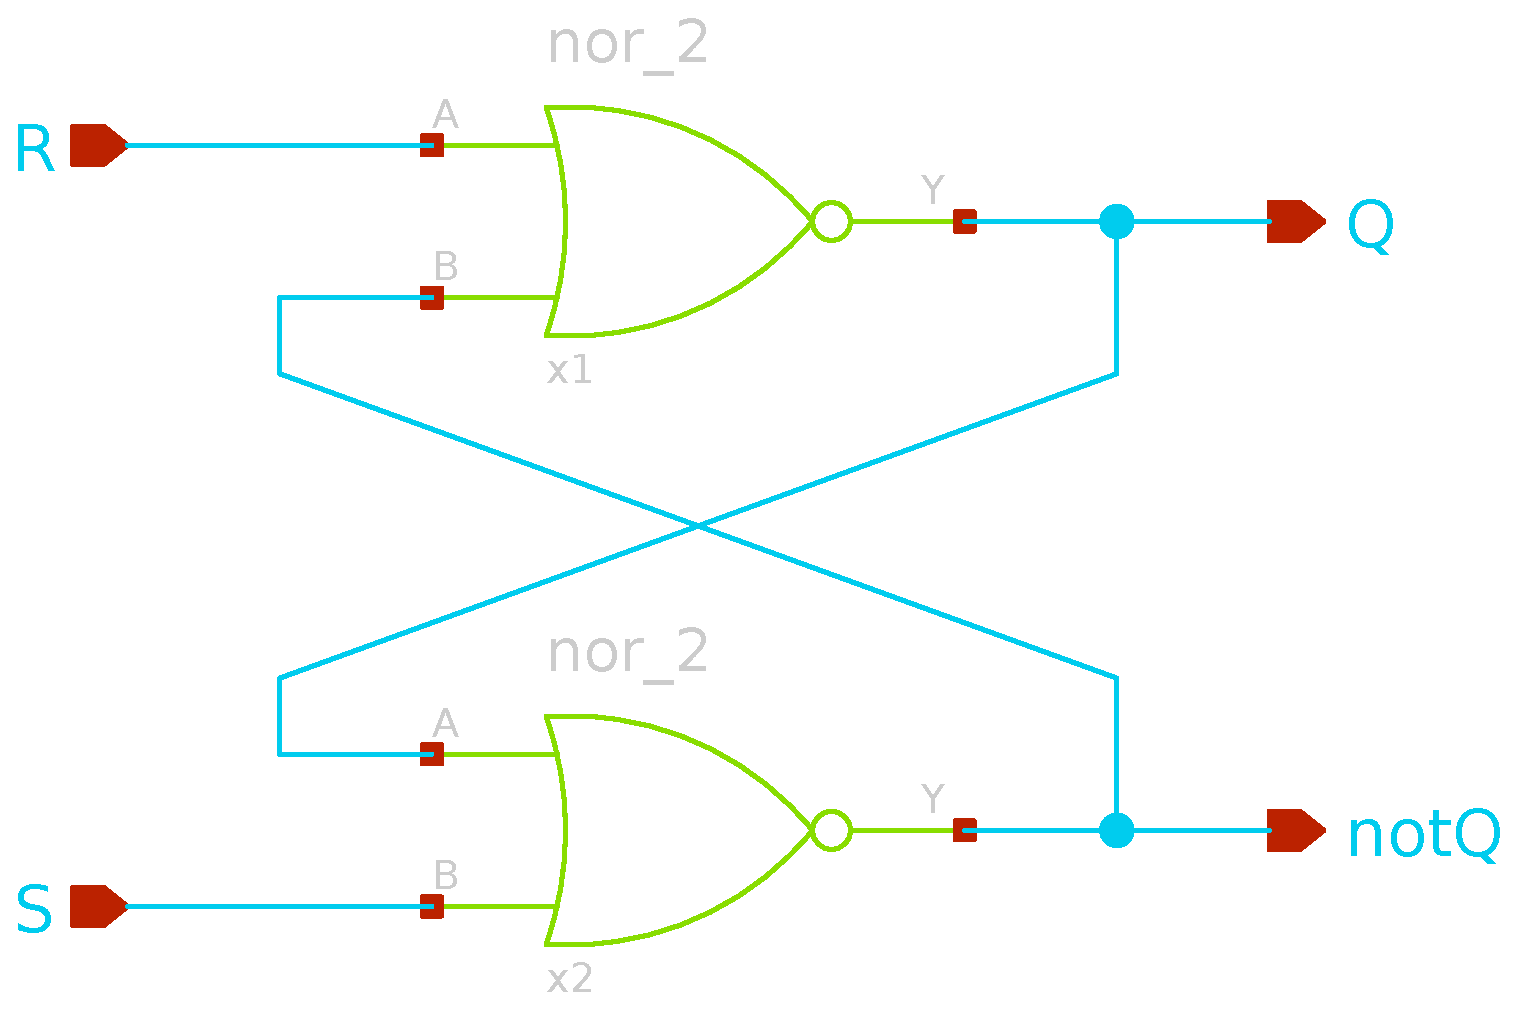
\includegraphics[width=5cm]{Immagini/srlatch-sch} \caption{}
		\end{subfigure}
		\begin{subfigure}{0.48\linewidth}
			\centering
			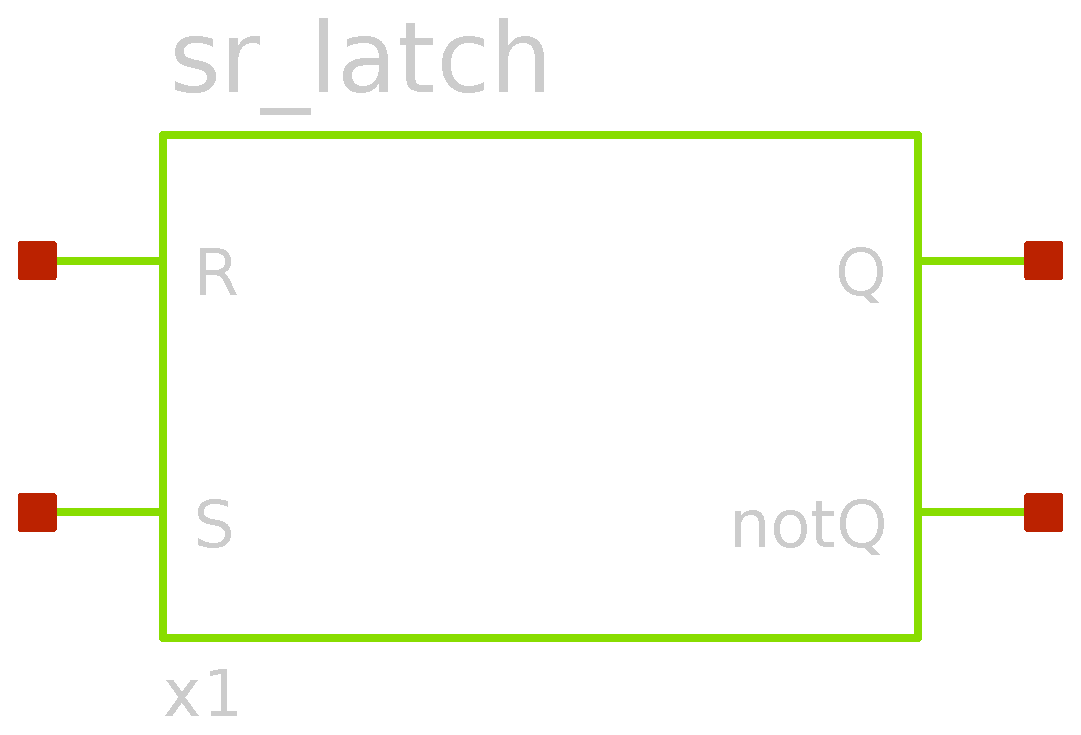
\includegraphics[width=3cm]{Immagini/srlatch-simple} \caption{}
		\end{subfigure}
		\caption{implementazione circuitale di un latch SR (a) e relativa rappresentazione schematica semplificata (b).}
		\label{fig:srl:schematico}
	\end{figure}
	
	Costruendo la tabella \ref{tab:srl:tabellaverita} di verità di questo tipo di latch è possibile descrivere l'uscita, generalmente indicata con $Q$, del dispositivo: nel caso venga imposto un segnale alto al terminale di $S$ allora anche l'uscita viene impostata (funzione di \textit{set}) alla tensione di alimentazione, mentre se viene imposto un segnale alto al terminale $R$ l'uscita viene ripristinata (funzione di \textit{reset}) alla tensione di massa. \\
	Nel caso in cui nessuno dei due terminali d'ingresso si trovi allo stato alto, ossia non sia specificata nessuna tra le azioni di set o reset, allora la retroazione garantisce un'uscita che rimane invariata allo stato precedente del sistema. Condizione di ingresso invalida per il sistema è invece quella per cui entrambi gli ingressi $S$ ed $R$ si trovano ad uno stato logico alto: in questo caso sia l'uscita $Q$ che il suo negato $\overline Q$ risultano poste allo stato logico basso (non verificando la disuguaglianza $Q\neq \overline Q$). Partendo dal presupposto che tale condizione a livello pratico non dovrebbe mai avvenire, in quanto non ha senso impostare e ripristinare lo stesso segnale contemporaneamente, il circuito ritorna ad uno stato funzionale "stabile" e di corretto funzionamento non appena uno dei segnali viene riportato ad un valore logico basso.
	
	
	\begin{table}[bht]
		\centering
		\begin{tabular}{c c | c c  l}
			$S$ & $R$ & $Q$ & $\overline Q$ \\ \hline
			0 & 0 & $\backsim$ & $\backsim$ \\
			0 & 1 & 0 & 1 \\
			1 & 0 & 1 & 0 \\
			1 & 1 & 0 & 0 & stato invalido 			
		\end{tabular}
		\caption{tabella di verità del latch SR. Con $\backsim$ si indica che lo stato del segnale rimane invariato rispetto al valore che aveva precedentemente acquisito.}
		\label{tab:srl:tabellaverita}
	\end{table}
	
	Il principio di funzionamento del latch SR è dovuto alla natura della porta logica nor che lo compone, e si basa sul fatto che l'uscita del circuito è alta solamente se entrambi gli ingressi si trovano ad uno stato basso. Il collegamento in retroazione che determina l'ingresso di un gate con l'uscita dell'altro permette di espletare la funzione per cui solamente una delle due uscite può essere alta contemporaneamente nel caso in cui gli ingressi siano ad uno stato logico basso. Forzando invece un ingresso (per esempio $S$) allo stato logico alto, allora si impone che l'uscita del gate associato (in questo caso $\overline Q$) venga posta a 0: il gate complementare (associato all'ingresso $R$) osserverà così entrambi gli ingressi bassi ponendo l'uscita $Q$ allo stato logico alto.\\
	A questo punto anche se si rimuovesse l'ingresso $S$ alto, lo stato del circuito rimarrebbe invariato in quanto il gate associato a tale terminale risulterebbe attivato dalla retroazione dovuta al segnale $Q$ che è alto. Si può analizzare la commutazione del circuito nel caso di segnale di reset alto in modo speculare.
	
	\begin{figure}[H]
		\centering
		\input{Immagini/srlatch-sim}
		\caption{rappresentazione dell'andamento del tempo del segnale d'uscita $Q$ e del suo negato $\overline Q$ in funzione degli impulsi di set e di reset. Le uscite sono state collegate a massa con una capacità di carico di $0.75pF$ rappresentativa del circuito a valle del latch SR.}
		\label{fig:srl:transitorio}
	\end{figure}

	In figura \ref{fig:srl:transitorio} è rappresentato l'andamento nel tempo delle uscite del circuito in funzione di impulsi in ingresso ai segnali di set e reset. Si può osservare che fino al primo impulso le uscite non sono ben definite, e questo è dovuto alla non inizializzazione del circuito. Nel caso ideale ottenuto mediante simulazione le uscite si trovano ad una tensione $V_{dd}/2$, tuttavia nel caso reale un'uscita prevarrebbe sull'altra per stato logico per via delle imperfezioni di realizzazione dei transistor (per esempio i rapporti $W/L$ o la conducibilità intrinseca potrebbero differire leggermente tra i transistor che compongono i gate, portando ad uno sbilanciamento del circuito), determinando un'uscita iniziale generalmente ignota.
	
	Va inoltre osservato che il segnale alto in ingresso deve rimanere in tale stato per un tempo necessario a garantire la rispettiva commutazione dell'uscita, pena la non corretta funzionalità del circuito stesso. Considerando la capacità di carico di $0.75pF$ il valore dell'impulso alto deve essere al minimo pari a $t_{min} = 7.28ns$. 

\subsection*{SR latch con segnale di \textit{enable}}
	Spesso i circuiti digitali sono predisposti con dei cosiddetti segnali di \textit{enable}, ossia di abilitazione degli ingressi. Questo significa che è possibile specificare al dispositivo quando lo stesso può leggere i segnali in ingresso oppure ignorarli.
	
	Sfruttando la convenzione per la quale il segnale di abilitazione è attivo quando il rispettivo stato logico è alto, è possibile creare un latch SR con funzione di enable anteponendo agli ingressi $S,R$ dei gate nor delle porte nand, come in figura \ref{fig:srl:schematico-enable}.
	
	\begin{figure}[bht]
		\centering
		\begin{subfigure}{0.48\linewidth}
			\centering
			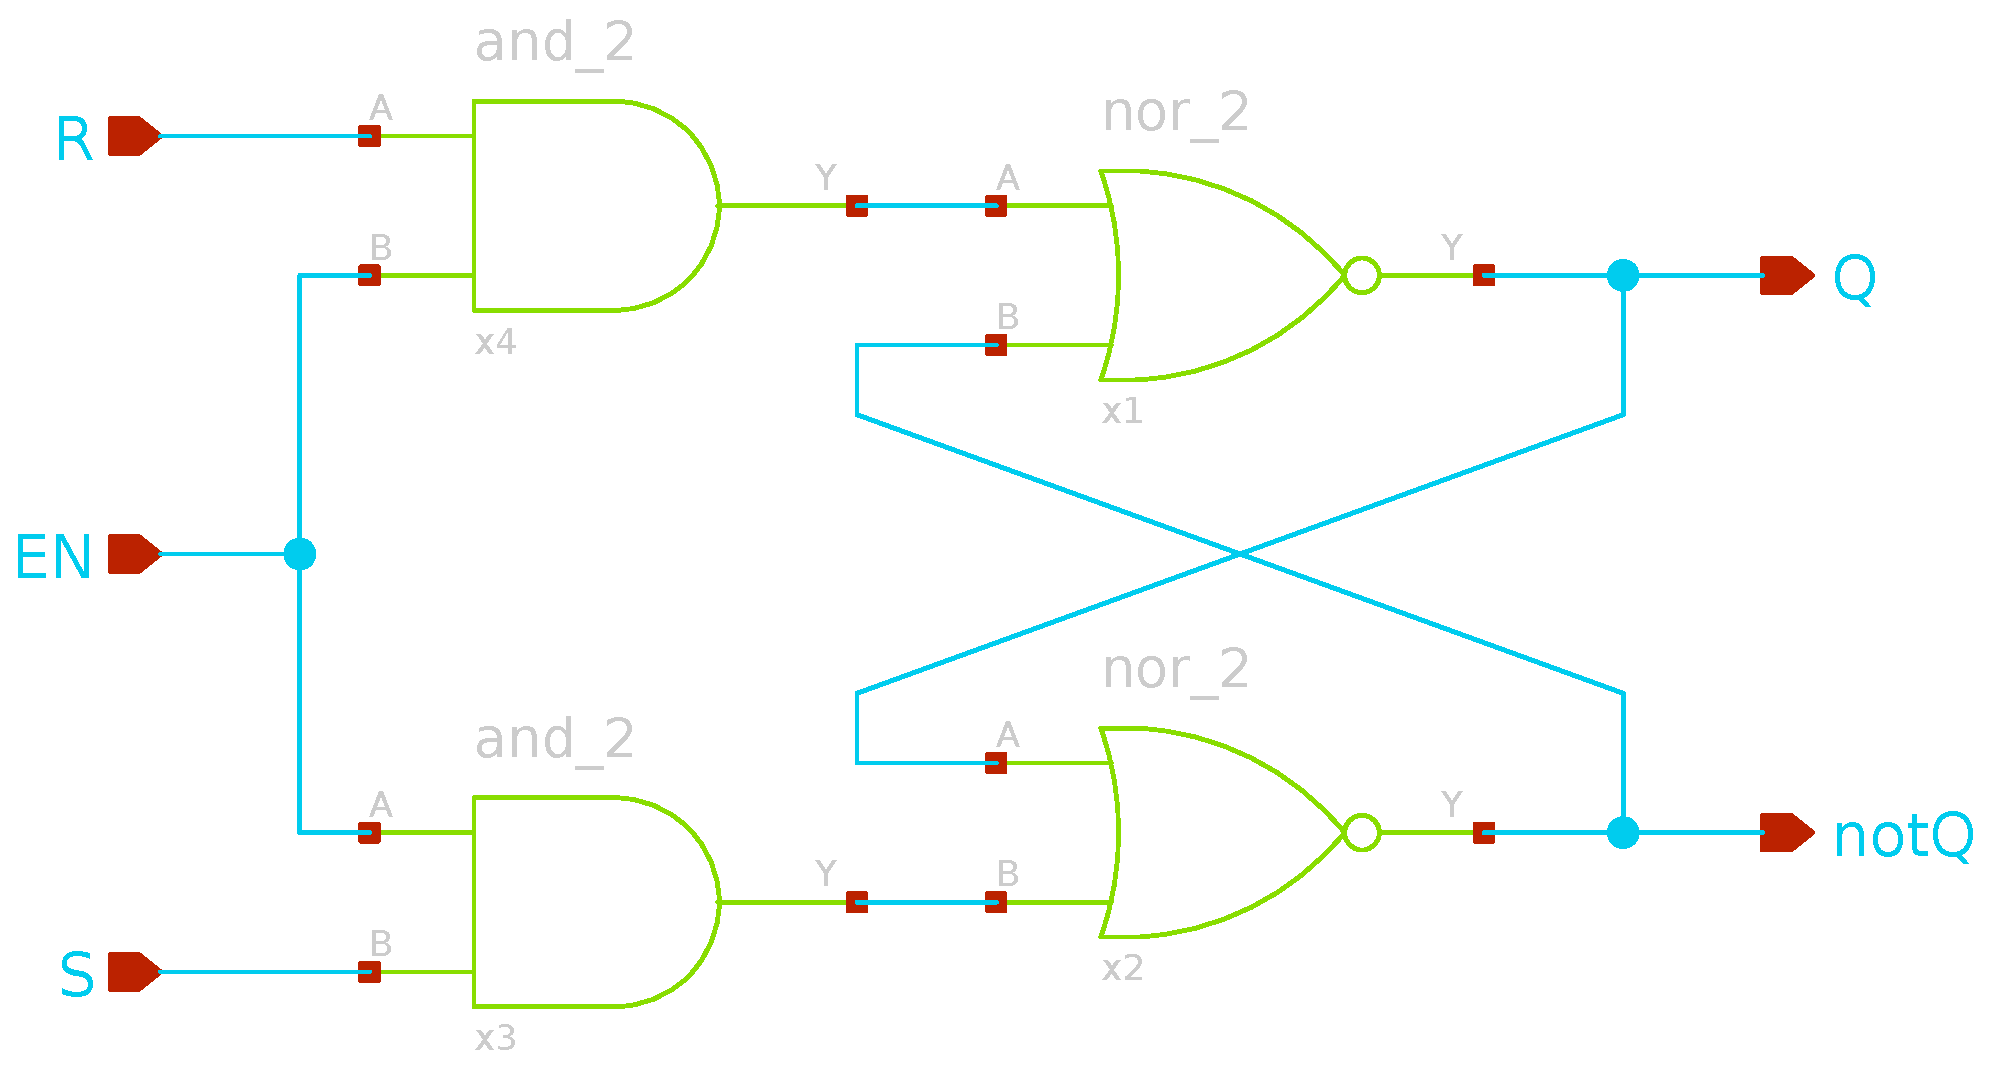
\includegraphics[width=6.5cm]{Immagini/srlatch-en-sch} \caption{}
		\end{subfigure}
		\begin{subfigure}{0.48\linewidth}
			\centering
			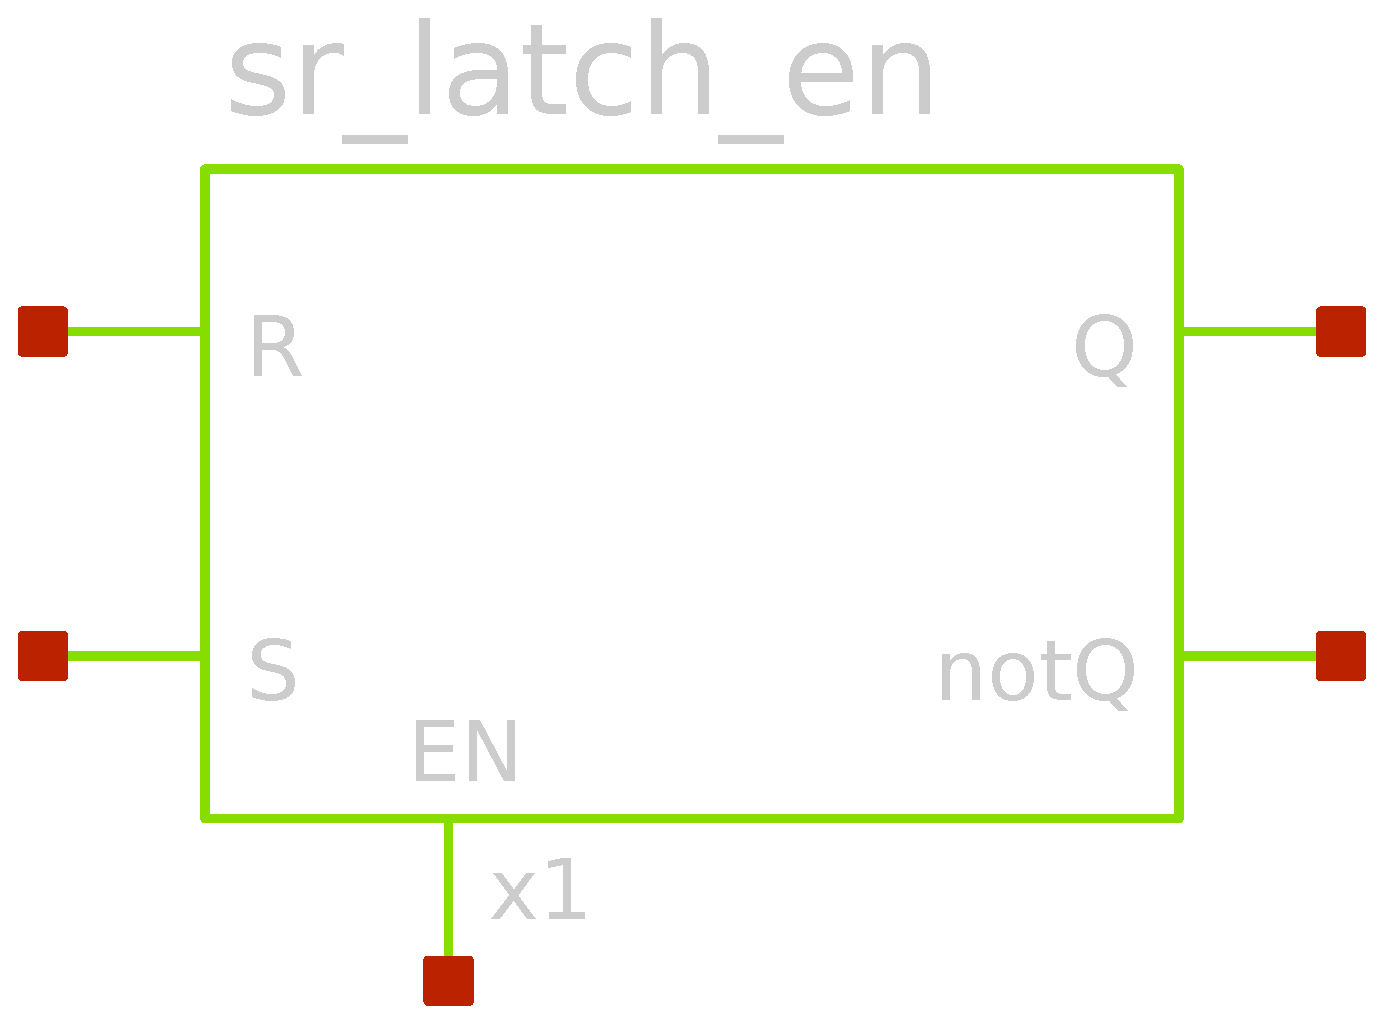
\includegraphics[width=3cm]{Immagini/srlatch-en-simple} \caption{}
		\end{subfigure}
		\caption{implementazione circuitale di un latch SR con ingresso di enable (a) e relativa rappresentazione schematica semplificata (b).}
		\label{fig:srl:schematico-enable}
	\end{figure}
	
	In questo caso gli ingressi $S,R$ possono essere processati dal latch solamente se il segnale di enable è alto; nel caso in cui il segnale di abilitazione sia basso, allora gli ingressi che giungerebbero al latch sarebbero entrambi 0, con conseguente invarianza dell'uscita.

	In figura \ref{fig:srl:transitorio-enable} è possibile osservare come cambia la risposta di questa variante del latch SR, mantenendo inalterati i segnali di set e reset in ingresso.
	
	\begin{figure}[bht]
		\centering
		\input{Immagini/srlatch-en-sim}
		\caption{rappresentazione dell'andamento del tempo del segnale d'uscita $Q$ in funzione degli impulsi di set e reset, considerando inoltre il segnale di abilitazione $EN$. Le uscite del latch state collegate a massa con una capacità di carico di $0.
		75V$ rappresentativa del circuito a valle. Tutti i valori lungo l'asse delle ordinate sono da ritenersi in volt.}
		\label{fig:srl:transitorio-enable}
	\end{figure}
	
	Si osserva così che solo i primi impulsi di set e reset determinano una variazione dell'uscita del latch, in quanto sono gli unici segnali all'interno della fascia temporale del segnale di enable allo stato alto. Al tempo $t=65ns$ il segnale di abilitazione scende al valore logico basso, e dunque ignora il successivo segnale di reset (che pertanto non influenza l'uscita del latch).
	
\subsection*{SR flip-flop}
	Una caratteristica fondamentale che caratterizza tutti i circuiti digitali per migliorarne l'efficienza e la stabilità è il sincronismo: in ogni circuito integrato infatti è possibile trovare un generatore di sincronismo che invia (ad una frequenza prestabilita) i segnali di \textit{clock}. Questi elementi, realizzati solitamente tramite circuiti astabili, generano di fatto delle onde quadre di periodo costante e pre-determinato (individuato dalla risonanza di elementi ceramici o dalle costanti di tempo di filtri RC) del quale è anche possibile stabilire il duty cycle, ossia la percentuale di tempo del segnale alto rispetto al periodo complessivo.
	
	La transizione del segnale da basso ad alto (o viceversa) determina il sincronismo tra tutti i gli elementi collegati al circuito stesso, determinando con cadenza regolare quando procedere con le operazioni successive.
	
	Analizzando il latch SR con enable descritto in precedenza, l'elemento di sincronismo può essere introdotto proprio nel segnale di abilitazione del circuito digitale stesso. Un problema che si osserva è che tuttavia questo elemento di memoria, allo stato attuale, commuta l'uscita in funzione degli impulsi di set-reset che avvengono fintanto che il segnale di clock risulta essere alto.
	
	Si introduce dunque la necessità di individuare dei circuiti \textit{edge detector} che permettono di rilevare le transizioni del segnale di clock e alle quali si associano degli impulsi (come delle onde quadre) con tempo in stato logico alto di durata molto bassa. Sfruttando questi circuiti è possibile garantire la lettura agli ingressi $S$ ed $R$ del latch solamente nell'intervallo di tempo in cui si ha la commutazione del segnale. Il circuito edge detector deve inoltre garantire un tempo di segnale alto in uscita che sia sufficiente per gli ingressi a pilotare il circuito a valle.
	
	\begin{figure}[bht]
		\centering
		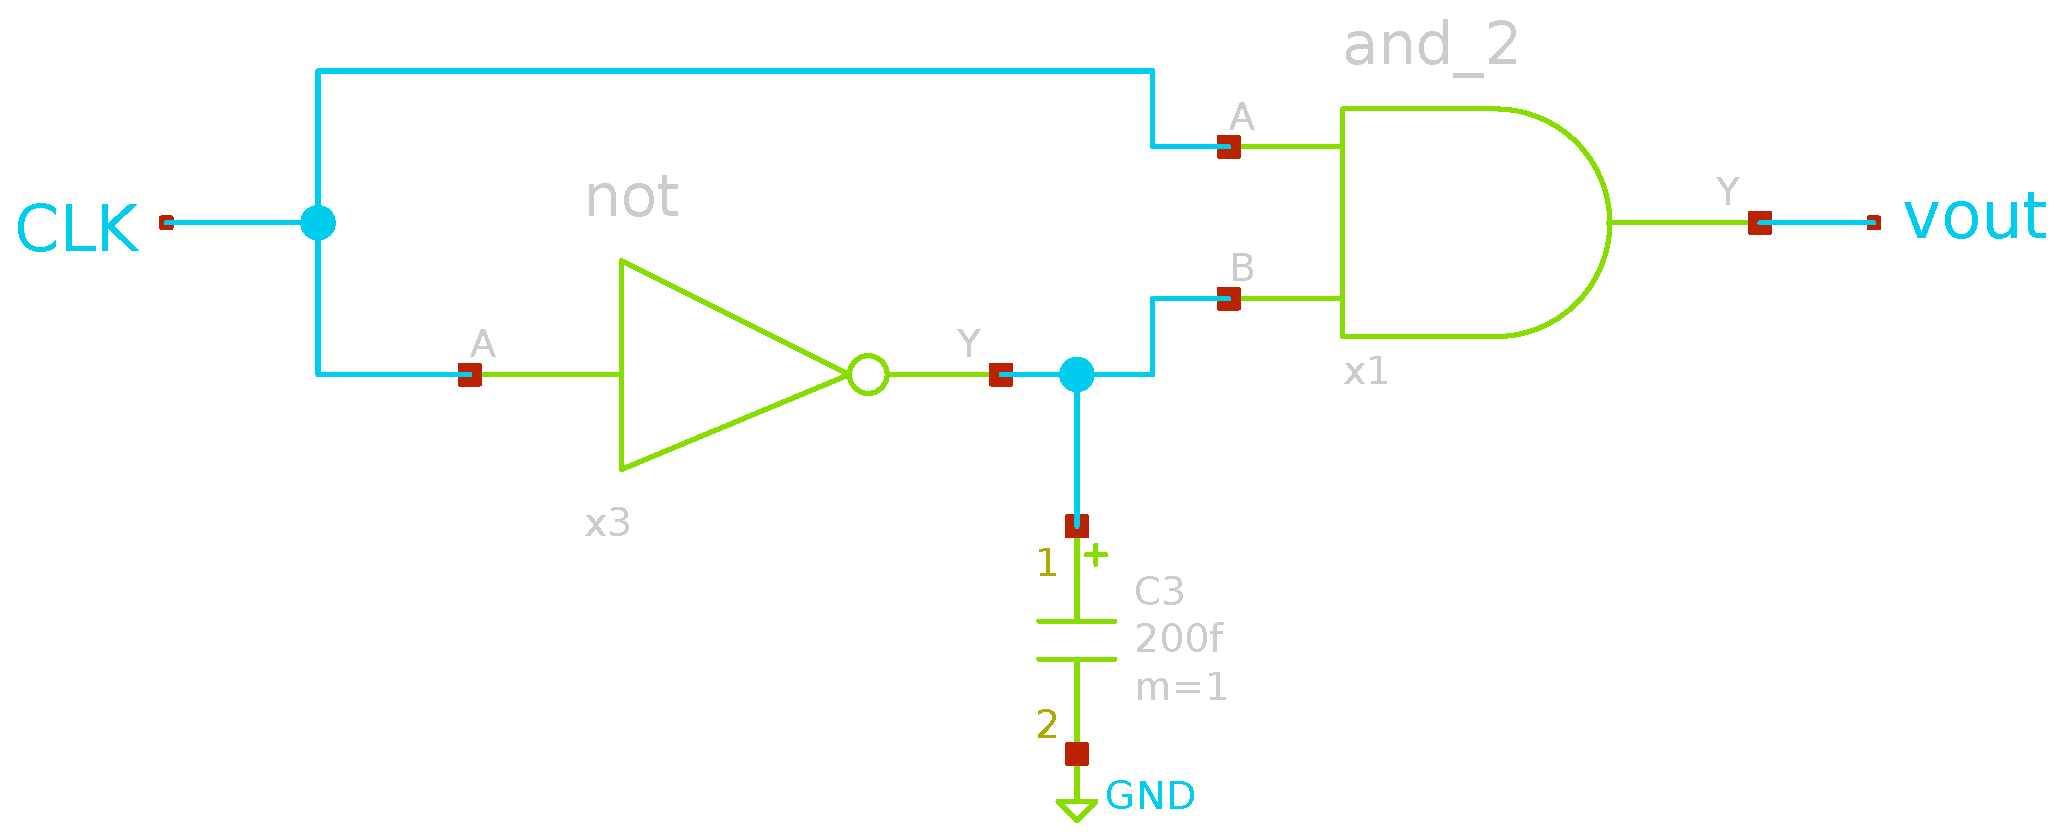
\includegraphics[width=6cm]{Immagini/edge-detector}
		\caption{implementazione circuitale di un edge detector che rileva la commutazione dell'ingresso da basso a alto.}
		\label{fig:srl:edgedetector}
	\end{figure}
	
	Un circuito che si può realizzare semplicemente mediante l'interconnessione di gate logici è l'edge detector mostrato in figura \ref{fig:srl:edgedetector}, composto da un invertitore logico e da una porta and.\\
	Nonostante ci si aspetta che l'uscita di tale circuito sia sempre bassa (in quanto il prodotto logico tra un segnale e il suo negato è sempre basso), la presenza delle capacità nei gate logici (e in questo caso è aggiunta anche una capacità supplementare di $1.5pF$) determinano un ritardo nella commutazione dell'invertitore. Considerando il fronte di salita del segnale di clock, gli ingressi al gate and saranno entrambi alti in quanto l'invertitore necessiterà di una determinata quantità di tempo per invertire la tensione alla sua uscita, dovendo anche scaricare la relativa capacità.
	\begin{figure}[bht]
		\centering
		% GNUPLOT: LaTeX picture with Postscript
\begingroup
  \makeatletter
  \providecommand\color[2][]{%
    \GenericError{(gnuplot) \space\space\space\@spaces}{%
      Package color not loaded in conjunction with
      terminal option `colourtext'%
    }{See the gnuplot documentation for explanation.%
    }{Either use 'blacktext' in gnuplot or load the package
      color.sty in LaTeX.}%
    \renewcommand\color[2][]{}%
  }%
  \providecommand\includegraphics[2][]{%
    \GenericError{(gnuplot) \space\space\space\@spaces}{%
      Package graphicx or graphics not loaded%
    }{See the gnuplot documentation for explanation.%
    }{The gnuplot epslatex terminal needs graphicx.sty or graphics.sty.}%
    \renewcommand\includegraphics[2][]{}%
  }%
  \providecommand\rotatebox[2]{#2}%
  \@ifundefined{ifGPcolor}{%
    \newif\ifGPcolor
    \GPcolorfalse
  }{}%
  \@ifundefined{ifGPblacktext}{%
    \newif\ifGPblacktext
    \GPblacktexttrue
  }{}%
  % define a \g@addto@macro without @ in the name:
  \let\gplgaddtomacro\g@addto@macro
  % define empty templates for all commands taking text:
  \gdef\gplbacktext{}%
  \gdef\gplfronttext{}%
  \makeatother
  \ifGPblacktext
    % no textcolor at all
    \def\colorrgb#1{}%
    \def\colorgray#1{}%
  \else
    % gray or color?
    \ifGPcolor
      \def\colorrgb#1{\color[rgb]{#1}}%
      \def\colorgray#1{\color[gray]{#1}}%
      \expandafter\def\csname LTw\endcsname{\color{white}}%
      \expandafter\def\csname LTb\endcsname{\color{black}}%
      \expandafter\def\csname LTa\endcsname{\color{black}}%
      \expandafter\def\csname LT0\endcsname{\color[rgb]{1,0,0}}%
      \expandafter\def\csname LT1\endcsname{\color[rgb]{0,1,0}}%
      \expandafter\def\csname LT2\endcsname{\color[rgb]{0,0,1}}%
      \expandafter\def\csname LT3\endcsname{\color[rgb]{1,0,1}}%
      \expandafter\def\csname LT4\endcsname{\color[rgb]{0,1,1}}%
      \expandafter\def\csname LT5\endcsname{\color[rgb]{1,1,0}}%
      \expandafter\def\csname LT6\endcsname{\color[rgb]{0,0,0}}%
      \expandafter\def\csname LT7\endcsname{\color[rgb]{1,0.3,0}}%
      \expandafter\def\csname LT8\endcsname{\color[rgb]{0.5,0.5,0.5}}%
    \else
      % gray
      \def\colorrgb#1{\color{black}}%
      \def\colorgray#1{\color[gray]{#1}}%
      \expandafter\def\csname LTw\endcsname{\color{white}}%
      \expandafter\def\csname LTb\endcsname{\color{black}}%
      \expandafter\def\csname LTa\endcsname{\color{black}}%
      \expandafter\def\csname LT0\endcsname{\color{black}}%
      \expandafter\def\csname LT1\endcsname{\color{black}}%
      \expandafter\def\csname LT2\endcsname{\color{black}}%
      \expandafter\def\csname LT3\endcsname{\color{black}}%
      \expandafter\def\csname LT4\endcsname{\color{black}}%
      \expandafter\def\csname LT5\endcsname{\color{black}}%
      \expandafter\def\csname LT6\endcsname{\color{black}}%
      \expandafter\def\csname LT7\endcsname{\color{black}}%
      \expandafter\def\csname LT8\endcsname{\color{black}}%
    \fi
  \fi
    \setlength{\unitlength}{0.0500bp}%
    \ifx\gptboxheight\undefined%
      \newlength{\gptboxheight}%
      \newlength{\gptboxwidth}%
      \newsavebox{\gptboxtext}%
    \fi%
    \setlength{\fboxrule}{0.5pt}%
    \setlength{\fboxsep}{1pt}%
\begin{picture}(5668.00,2266.00)%
    \gplgaddtomacro\gplbacktext{%
      \csname LTb\endcsname%%
      \put(434,1377){\makebox(0,0)[r]{\strut{}$0$}}%
      \csname LTb\endcsname%%
      \put(434,1767){\makebox(0,0)[r]{\strut{}$0.9$}}%
      \csname LTb\endcsname%%
      \put(434,2156){\makebox(0,0)[r]{\strut{}$1.8$}}%
      \csname LTb\endcsname%%
      \put(566,1071){\makebox(0,0){\strut{}}}%
      \csname LTb\endcsname%%
      \put(1369,1071){\makebox(0,0){\strut{}}}%
      \csname LTb\endcsname%%
      \put(2172,1071){\makebox(0,0){\strut{}}}%
      \csname LTb\endcsname%%
      \put(2975,1071){\makebox(0,0){\strut{}}}%
      \csname LTb\endcsname%%
      \put(3777,1071){\makebox(0,0){\strut{}}}%
      \csname LTb\endcsname%%
      \put(4580,1071){\makebox(0,0){\strut{}}}%
      \csname LTb\endcsname%%
      \put(5383,1071){\makebox(0,0){\strut{}}}%
    }%
    \gplgaddtomacro\gplfronttext{%
      \csname LTb\endcsname%%
      \put(-171,1766){\rotatebox{-270}{\makebox(0,0){\strut{}$V_{out}$}}}%
      \put(2974,1005){\makebox(0,0){\strut{}}}%
    }%
    \gplgaddtomacro\gplbacktext{%
      \csname LTb\endcsname%%
      \put(434,426){\makebox(0,0)[r]{\strut{}$0$}}%
      \csname LTb\endcsname%%
      \put(434,815){\makebox(0,0)[r]{\strut{}$0.9$}}%
      \csname LTb\endcsname%%
      \put(434,1204){\makebox(0,0)[r]{\strut{}$1.8$}}%
      \csname LTb\endcsname%%
      \put(566,119){\makebox(0,0){\strut{}0}}%
      \csname LTb\endcsname%%
      \put(1369,119){\makebox(0,0){\strut{}10}}%
      \csname LTb\endcsname%%
      \put(2172,119){\makebox(0,0){\strut{}20}}%
      \csname LTb\endcsname%%
      \put(2975,119){\makebox(0,0){\strut{}30}}%
      \csname LTb\endcsname%%
      \put(3777,119){\makebox(0,0){\strut{}40}}%
      \csname LTb\endcsname%%
      \put(4580,119){\makebox(0,0){\strut{}50}}%
      \csname LTb\endcsname%%
      \put(5383,119){\makebox(0,0){\strut{}60}}%
    }%
    \gplgaddtomacro\gplfronttext{%
      \csname LTb\endcsname%%
      \put(-171,815){\rotatebox{-270}{\makebox(0,0){\strut{}$CLK$}}}%
      \put(2974,-211){\makebox(0,0){\strut{}tempo $[ns]$}}%
    }%
    \gplbacktext
    \put(0,0){\includegraphics[width={283.40bp},height={113.30bp}]{Immagini/edge-detector-sim}}%
    \gplfronttext
  \end{picture}%
\endgroup


		\vspace{3mm}
		\caption{risposta del circuito di edge detection ad un segnale di clock di periodo $30ns$ e duty cycle del $50\%$.}
		\label{fig:srl:edgesimulation}
	\end{figure}
	
	Come si può osservare dalla figura \ref{fig:srl:edgesimulation} questo circuito così realizzato permette di rilevare i fronti di salita del segnale di clock generano un relativo segnale alto per una durata di circa $8.9ns$, ossia il tempo generalmente necessario ai gate logici per effettuare delle eventuali commutazioni di segnali. Variando la capacità del circuito è possibile aumentare o diminuire il periodo di pulsazione dovuta al fronte di salita.
	
	\vspace{3mm}
	Avendo dunque determinato un circuito di edge detection è possibile implementare il \textit{flip-flop SR} (figura \ref{fig:srl:flipflop}), ossia un latch SR che sfrutta il circuito appena realizzato per commutare i suoi ingressi solamente in corrispondenza dei fronti di salita del segnale di clock.
	
	\begin{figure}[bht]
		\centering
		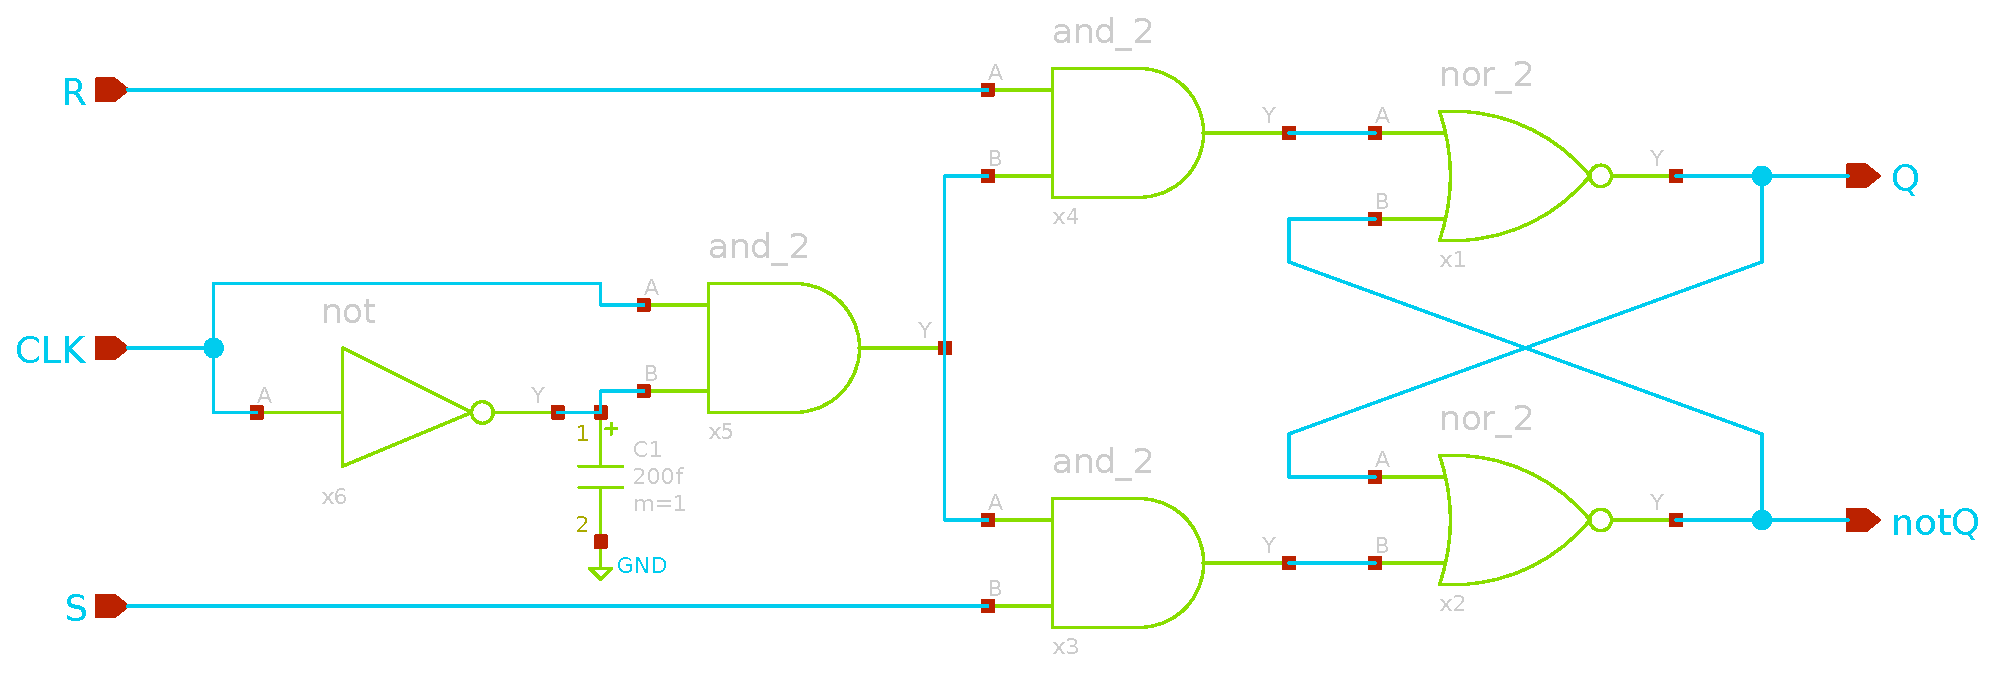
\includegraphics[width=9cm]{Immagini/srflipflop}
		\caption{implementazione circuitale di un flip-flop SR.}
		\label{fig:srl:flipflop}
	\end{figure}
	
	Effettuando delle simulazioni sui transitori (figura \ref{fig:srl:flipflop-sim}) è possibile infatti verificare il corretto funzionamento, come previsto, del circuito: il flip-flop commuta opportunamente la sua uscita in funzione dei segnali di set/reset solamente in presenza di un fronte positivo del segnale di clock.
	
	\begin{figure}[bht]
		\centering
		% GNUPLOT: LaTeX picture with Postscript
\begingroup
  \makeatletter
  \providecommand\color[2][]{%
    \GenericError{(gnuplot) \space\space\space\@spaces}{%
      Package color not loaded in conjunction with
      terminal option `colourtext'%
    }{See the gnuplot documentation for explanation.%
    }{Either use 'blacktext' in gnuplot or load the package
      color.sty in LaTeX.}%
    \renewcommand\color[2][]{}%
  }%
  \providecommand\includegraphics[2][]{%
    \GenericError{(gnuplot) \space\space\space\@spaces}{%
      Package graphicx or graphics not loaded%
    }{See the gnuplot documentation for explanation.%
    }{The gnuplot epslatex terminal needs graphicx.sty or graphics.sty.}%
    \renewcommand\includegraphics[2][]{}%
  }%
  \providecommand\rotatebox[2]{#2}%
  \@ifundefined{ifGPcolor}{%
    \newif\ifGPcolor
    \GPcolorfalse
  }{}%
  \@ifundefined{ifGPblacktext}{%
    \newif\ifGPblacktext
    \GPblacktexttrue
  }{}%
  % define a \g@addto@macro without @ in the name:
  \let\gplgaddtomacro\g@addto@macro
  % define empty templates for all commands taking text:
  \gdef\gplbacktext{}%
  \gdef\gplfronttext{}%
  \makeatother
  \ifGPblacktext
    % no textcolor at all
    \def\colorrgb#1{}%
    \def\colorgray#1{}%
  \else
    % gray or color?
    \ifGPcolor
      \def\colorrgb#1{\color[rgb]{#1}}%
      \def\colorgray#1{\color[gray]{#1}}%
      \expandafter\def\csname LTw\endcsname{\color{white}}%
      \expandafter\def\csname LTb\endcsname{\color{black}}%
      \expandafter\def\csname LTa\endcsname{\color{black}}%
      \expandafter\def\csname LT0\endcsname{\color[rgb]{1,0,0}}%
      \expandafter\def\csname LT1\endcsname{\color[rgb]{0,1,0}}%
      \expandafter\def\csname LT2\endcsname{\color[rgb]{0,0,1}}%
      \expandafter\def\csname LT3\endcsname{\color[rgb]{1,0,1}}%
      \expandafter\def\csname LT4\endcsname{\color[rgb]{0,1,1}}%
      \expandafter\def\csname LT5\endcsname{\color[rgb]{1,1,0}}%
      \expandafter\def\csname LT6\endcsname{\color[rgb]{0,0,0}}%
      \expandafter\def\csname LT7\endcsname{\color[rgb]{1,0.3,0}}%
      \expandafter\def\csname LT8\endcsname{\color[rgb]{0.5,0.5,0.5}}%
    \else
      % gray
      \def\colorrgb#1{\color{black}}%
      \def\colorgray#1{\color[gray]{#1}}%
      \expandafter\def\csname LTw\endcsname{\color{white}}%
      \expandafter\def\csname LTb\endcsname{\color{black}}%
      \expandafter\def\csname LTa\endcsname{\color{black}}%
      \expandafter\def\csname LT0\endcsname{\color{black}}%
      \expandafter\def\csname LT1\endcsname{\color{black}}%
      \expandafter\def\csname LT2\endcsname{\color{black}}%
      \expandafter\def\csname LT3\endcsname{\color{black}}%
      \expandafter\def\csname LT4\endcsname{\color{black}}%
      \expandafter\def\csname LT5\endcsname{\color{black}}%
      \expandafter\def\csname LT6\endcsname{\color{black}}%
      \expandafter\def\csname LT7\endcsname{\color{black}}%
      \expandafter\def\csname LT8\endcsname{\color{black}}%
    \fi
  \fi
    \setlength{\unitlength}{0.0500bp}%
    \ifx\gptboxheight\undefined%
      \newlength{\gptboxheight}%
      \newlength{\gptboxwidth}%
      \newsavebox{\gptboxtext}%
    \fi%
    \setlength{\fboxrule}{0.5pt}%
    \setlength{\fboxsep}{1pt}%
\begin{picture}(5668.00,3400.00)%
    \gplgaddtomacro\gplbacktext{%
      \csname LTb\endcsname%%
      \put(434,2717){\makebox(0,0)[r]{\strut{}$0$}}%
      \csname LTb\endcsname%%
      \put(434,3009){\makebox(0,0)[r]{\strut{}$0.9$}}%
      \csname LTb\endcsname%%
      \put(434,3300){\makebox(0,0)[r]{\strut{}$1.8$}}%
      \csname LTb\endcsname%%
      \put(566,2432){\makebox(0,0){\strut{}}}%
      \csname LTb\endcsname%%
      \put(1101,2432){\makebox(0,0){\strut{}}}%
      \csname LTb\endcsname%%
      \put(1636,2432){\makebox(0,0){\strut{}}}%
      \csname LTb\endcsname%%
      \put(2172,2432){\makebox(0,0){\strut{}}}%
      \csname LTb\endcsname%%
      \put(2707,2432){\makebox(0,0){\strut{}}}%
      \csname LTb\endcsname%%
      \put(3242,2432){\makebox(0,0){\strut{}}}%
      \csname LTb\endcsname%%
      \put(3777,2432){\makebox(0,0){\strut{}}}%
      \csname LTb\endcsname%%
      \put(4313,2432){\makebox(0,0){\strut{}}}%
      \csname LTb\endcsname%%
      \put(4848,2432){\makebox(0,0){\strut{}}}%
      \csname LTb\endcsname%%
      \put(5383,2432){\makebox(0,0){\strut{}}}%
    }%
    \gplgaddtomacro\gplfronttext{%
      \csname LTb\endcsname%%
      \put(-171,3008){\rotatebox{-270}{\makebox(0,0){\strut{}$V_{out}$}}}%
      \put(2974,2366){\makebox(0,0){\strut{}}}%
    }%
    \gplgaddtomacro\gplbacktext{%
      \csname LTb\endcsname%%
      \put(434,2002){\makebox(0,0)[r]{\strut{}$0$}}%
      \csname LTb\endcsname%%
      \put(434,2294){\makebox(0,0)[r]{\strut{}$0.9$}}%
      \csname LTb\endcsname%%
      \put(434,2586){\makebox(0,0)[r]{\strut{}$1.8$}}%
      \csname LTb\endcsname%%
      \put(566,1717){\makebox(0,0){\strut{}}}%
      \csname LTb\endcsname%%
      \put(1101,1717){\makebox(0,0){\strut{}}}%
      \csname LTb\endcsname%%
      \put(1636,1717){\makebox(0,0){\strut{}}}%
      \csname LTb\endcsname%%
      \put(2172,1717){\makebox(0,0){\strut{}}}%
      \csname LTb\endcsname%%
      \put(2707,1717){\makebox(0,0){\strut{}}}%
      \csname LTb\endcsname%%
      \put(3242,1717){\makebox(0,0){\strut{}}}%
      \csname LTb\endcsname%%
      \put(3777,1717){\makebox(0,0){\strut{}}}%
      \csname LTb\endcsname%%
      \put(4313,1717){\makebox(0,0){\strut{}}}%
      \csname LTb\endcsname%%
      \put(4848,1717){\makebox(0,0){\strut{}}}%
      \csname LTb\endcsname%%
      \put(5383,1717){\makebox(0,0){\strut{}}}%
    }%
    \gplgaddtomacro\gplfronttext{%
      \csname LTb\endcsname%%
      \put(-171,2294){\rotatebox{-270}{\makebox(0,0){\strut{}$CLK$}}}%
      \put(2974,1651){\makebox(0,0){\strut{}}}%
    }%
    \gplgaddtomacro\gplbacktext{%
      \csname LTb\endcsname%%
      \put(434,1289){\makebox(0,0)[r]{\strut{}$0$}}%
      \csname LTb\endcsname%%
      \put(434,1581){\makebox(0,0)[r]{\strut{}$0.9$}}%
      \csname LTb\endcsname%%
      \put(434,1872){\makebox(0,0)[r]{\strut{}$1.8$}}%
      \csname LTb\endcsname%%
      \put(566,1004){\makebox(0,0){\strut{}}}%
      \csname LTb\endcsname%%
      \put(1101,1004){\makebox(0,0){\strut{}}}%
      \csname LTb\endcsname%%
      \put(1636,1004){\makebox(0,0){\strut{}}}%
      \csname LTb\endcsname%%
      \put(2172,1004){\makebox(0,0){\strut{}}}%
      \csname LTb\endcsname%%
      \put(2707,1004){\makebox(0,0){\strut{}}}%
      \csname LTb\endcsname%%
      \put(3242,1004){\makebox(0,0){\strut{}}}%
      \csname LTb\endcsname%%
      \put(3777,1004){\makebox(0,0){\strut{}}}%
      \csname LTb\endcsname%%
      \put(4313,1004){\makebox(0,0){\strut{}}}%
      \csname LTb\endcsname%%
      \put(4848,1004){\makebox(0,0){\strut{}}}%
      \csname LTb\endcsname%%
      \put(5383,1004){\makebox(0,0){\strut{}}}%
    }%
    \gplgaddtomacro\gplfronttext{%
      \csname LTb\endcsname%%
      \put(-171,1580){\rotatebox{-270}{\makebox(0,0){\strut{}$S$}}}%
      \put(2974,938){\makebox(0,0){\strut{}}}%
    }%
    \gplgaddtomacro\gplbacktext{%
      \csname LTb\endcsname%%
      \put(434,575){\makebox(0,0)[r]{\strut{}$0$}}%
      \csname LTb\endcsname%%
      \put(434,867){\makebox(0,0)[r]{\strut{}$0.9$}}%
      \csname LTb\endcsname%%
      \put(434,1158){\makebox(0,0)[r]{\strut{}$1.8$}}%
      \csname LTb\endcsname%%
      \put(566,290){\makebox(0,0){\strut{}0}}%
      \csname LTb\endcsname%%
      \put(1101,290){\makebox(0,0){\strut{}20}}%
      \csname LTb\endcsname%%
      \put(1636,290){\makebox(0,0){\strut{}40}}%
      \csname LTb\endcsname%%
      \put(2172,290){\makebox(0,0){\strut{}60}}%
      \csname LTb\endcsname%%
      \put(2707,290){\makebox(0,0){\strut{}80}}%
      \csname LTb\endcsname%%
      \put(3242,290){\makebox(0,0){\strut{}100}}%
      \csname LTb\endcsname%%
      \put(3777,290){\makebox(0,0){\strut{}120}}%
      \csname LTb\endcsname%%
      \put(4313,290){\makebox(0,0){\strut{}140}}%
      \csname LTb\endcsname%%
      \put(4848,290){\makebox(0,0){\strut{}160}}%
      \csname LTb\endcsname%%
      \put(5383,290){\makebox(0,0){\strut{}180}}%
    }%
    \gplgaddtomacro\gplfronttext{%
      \csname LTb\endcsname%%
      \put(-171,866){\rotatebox{-270}{\makebox(0,0){\strut{}$R$}}}%
      \put(2974,-40){\makebox(0,0){\strut{}tempo $[ns]$}}%
    }%
    \gplbacktext
    \put(0,0){\includegraphics[width={283.40bp},height={170.00bp}]{Immagini/sr-flipflop-sim}}%
    \gplfronttext
  \end{picture}%
\endgroup


		\caption{risposta dell'uscita di un flip-flop SR. Il circuito a valle è modellato da una capacità di $0.75pF$. Le tensioni sono espresse in volt.}
		\label{fig:srl:flipflop-sim}
	\end{figure}

\section{JK flip-flop}
	Un problema del latch SR e dei circuiti da esso derivati è l'invalidità dello stato con entrambi gli ingressi alti (come si osserva nell'ultima riga della tabella di verità \ref{tab:srl:tabellaverita} a pagina \pageref{tab:srl:tabellaverita}). Questo inconveniente rende il circuito instabile rispetto a ingressi contemporaneamente alti (in quanto non è possibile stabilire in maniera deterministica il funzionamento del circuito stesso nel momento in cui verranno tolti gli ingressi) e limita l'applicabilità di questo sistema di memoria.
	
	Per risolvere questo problema è stato inventato il \textit{flip-flop JK} i cui ingressi sono comunemente indicati dalle lettere J (associato alla funzione set) e K (associato alla funzione di reset). Come indicato nella tabella di verità \ref{tab:jkl:tabellaverita}, il comportamento generale del circuito rimane invariato se non nel caso di presenza di due ingressi alti contemporaneamente, momento nel quale le uscite $Q$ e $\overline Q$ commutano rispettivamente i loro stati da alto a basso e viceversa. 
	
	\begin{table}[bht]
		\centering
		\begin{tabular}{c c | c c }
			$S$ & $R$ & $Q$ & $\overline Q$ \\ \hline
			0 & 0 & $\backsim$ & $\backsim$ \\
			0 & 1 & 0 & 1 \\
			1 & 0 & 1 & 0 \\
			1 & 1 & \multicolumn{2}{c}{commutazione} 		
		\end{tabular}
		\caption{tabella di verità dei latch e flip-flop JK. Con $\backsim$ si indica che lo stato del segnale rimane invariato rispetto al valore che aveva precedentemente acquisito.}
		\label{tab:jkl:tabellaverita}
	\end{table}
	
	Tale effetto viene ottenuto retroazionando l'uscita dei gate nor con un terzo ingresso agli and di abilitazione del segnale (oltre che alla retroazione al gate nor stesso), come si può osservare in figura \ref{fig:jkff:schema}
	
	\begin{figure}[bht]
		\centering
		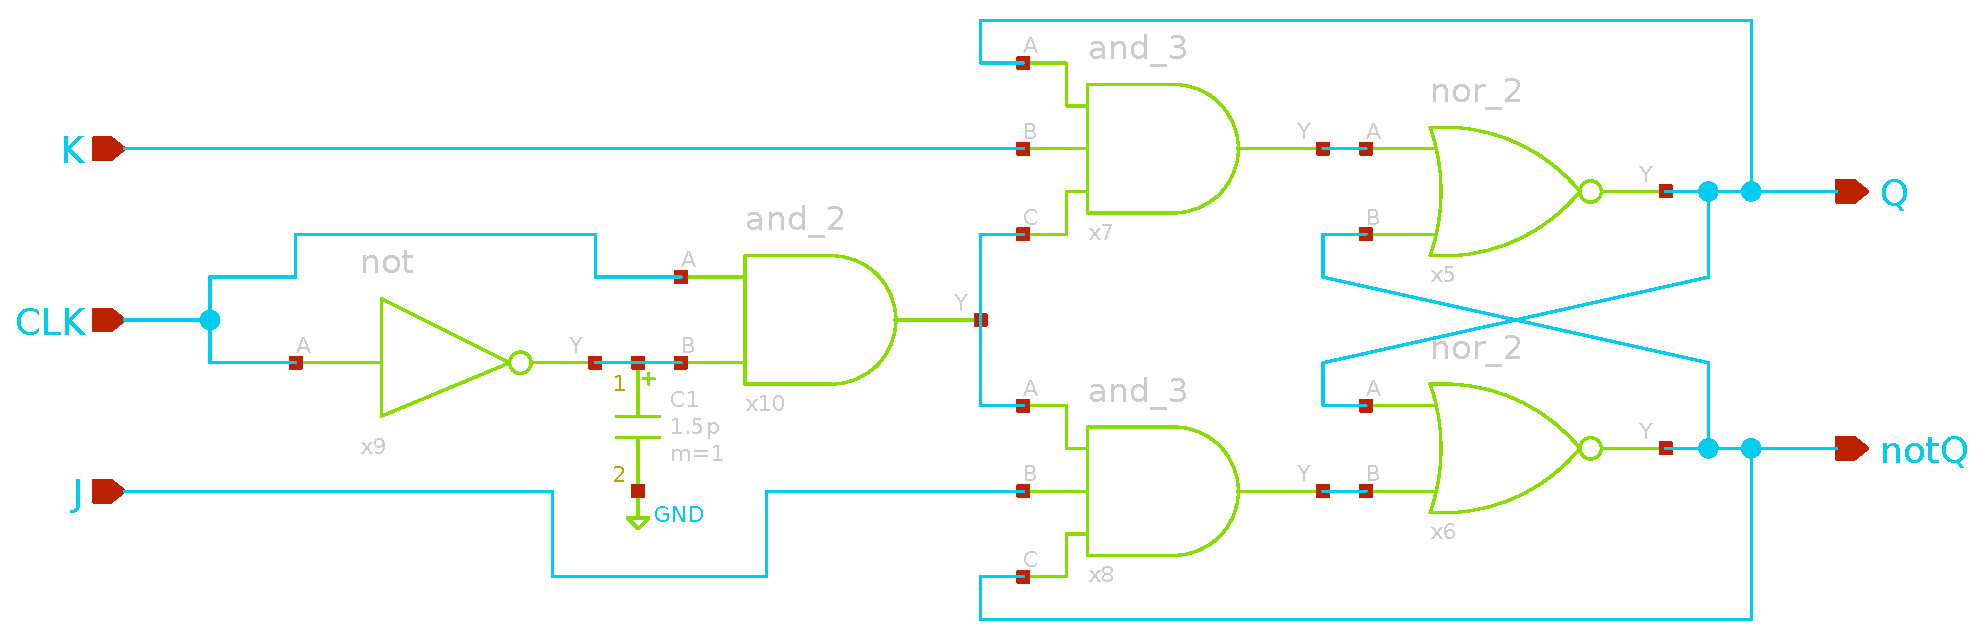
\includegraphics[width=8.5cm]{Immagini/jk-flipflop}
		\caption{implementazione circuitale di un flip-flop JK. Essendo il circuito un flip-flop, il segnale di clock viene opportunamente filtrato dall'edge detector.}
		\label{fig:jkff:schema}
	\end{figure}
	Tale realizzazione permette infatti di eliminare la possibilità di tensione alta agli ingressi di set e reset del latch SR che lo compone, ma solamente l'azione complementare all'uscita può essere realizzata. Per esempio se l'uscita si trovasse allo stato logico alto, solamente l'ingresso di reset potrà essere potrà essere attivato per commutare l'uscita.
	
	Simulando il circuito nel dominio del tempo è possibile verificare il funzionamento del flip-flop, osservando che l'implementazione (per come attualmente realizzata) presenta un problema critico nella commutazione.
	
	\begin{figure}[bht]
		\centering
		\input{Immagini/jkff-sim}
		\caption{risposta di un flip-flop JK; il circuito a valle è modellato da una capacità di $0.75pF$. Le tensioni sono espresse in volt.}
		\label{fig:jkff:sim-instabile}
	\end{figure}
	
	Rispetto ai risultati mostrati in figura \ref{fig:jkff:sim-instabile} per alcune commutazioni del segnale in uscita il transitorio non segue una funzione monotona, ma tende a oscillare per stabilizzarsi ad uno stato logico alto o basso (non necessariamente corretto rispetto all'ingresso del circuito) solamente quando il circuito di edge detection termina il suo segnale di abilitazione alto.
	
	Questo fenomeno prende il nome di \textit{gate racing} ed dovuto al fatto che i segnali in uscita $Q$ e $\overline Q$ sono retroazionati alla porta and di abilitazione dei segnali in ingresso: questo porta ad un rincorrersi delle uscite retroazionate che determinano l'instabilità critica del circuito per come così realizzato.
	
\subsection*{JK flip-flop master-slave}
	
	Per eliminare il problema di funzionamento critico del gate racing del flip-flop JK è possibile costruire una sua variante che prende il nome di \textit{master-slave} che è sostanzialmente composta da due flip-flop in sequenza. Come risulta evidente dell'implementazione circuitale (figura \ref{fig:jkff:masterslave}) il primo latch è detto master per via della sua funzione di interfacciamento con gli ingressi esterni, mentre il secondo (detto slave) è pilotato direttamente dal master.
	
	\begin{figure}[bht]
		\centering
		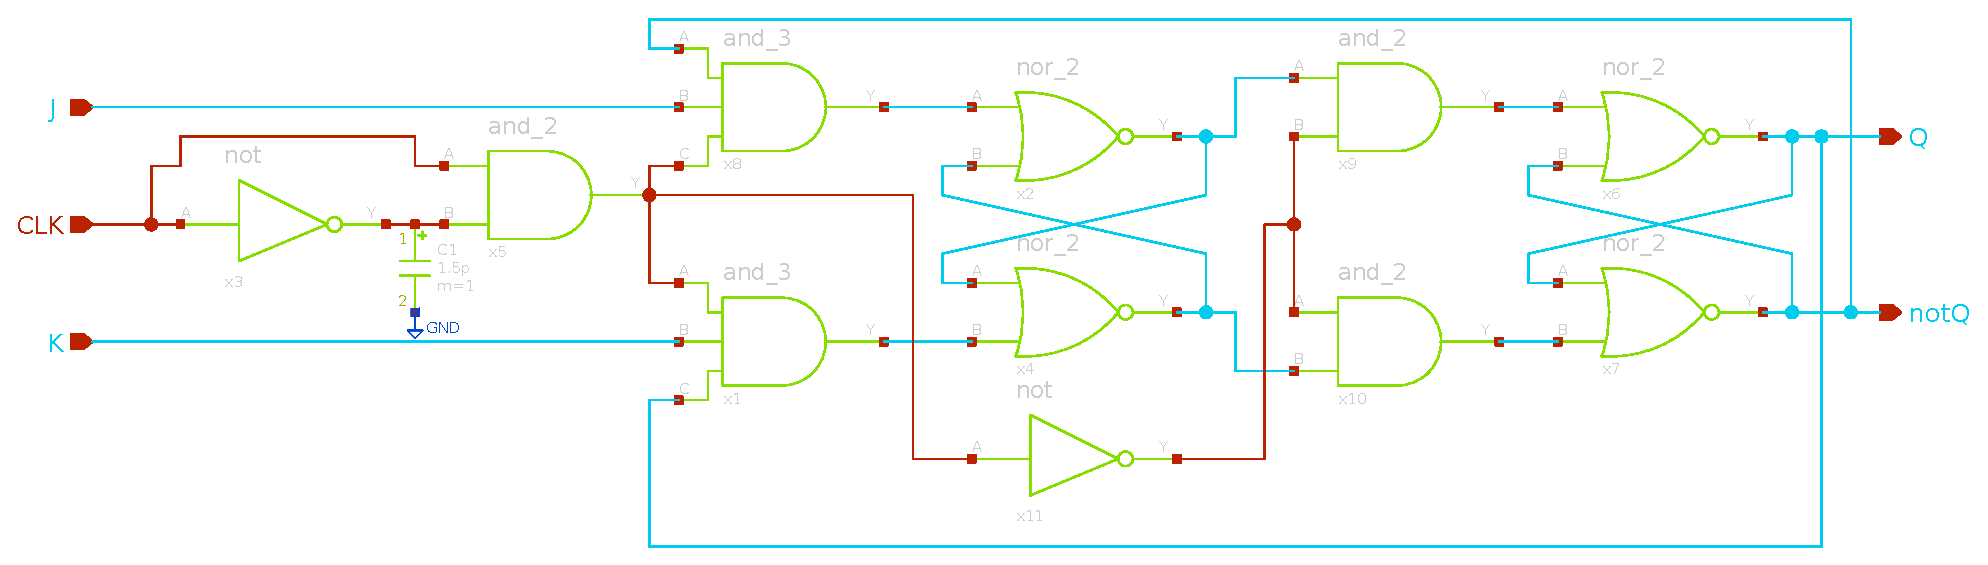
\includegraphics[width=12cm]{Immagini/jk-masterslave}
		\caption{implementazione circuitale di un flip-flop JK master-slave. Le connessioni in rosso evidenziano il circuito di clock.}
		\label{fig:jkff:masterslave}
	\end{figure}
	
	Il fenomeno del gate racing viene eliminato mediante l'implementazione di un circuito di abilitazione particolare per i due latch che compongono il circuito; infatti il segnale di clock (filtrato dal circuito di edge detection) viene utilizzato per abilitare il master del flip-flop, mentre per pilotare lo slave è necessario considerare il segnale negato. Questo significa che, allo stesso tempo, solo uno dei due latch può commutare (in quanto se un latch presenta uno stato di abilitazione alto, l'altro necessariamente lo osserverà basso).
	
	Questo introduce necessariamente un ritardo di commutazione dell'uscita, dipendente principalmente dal fronte alto generato dal circuito di edge detection in quanto tale impulso viene utilizzato per pilotare la prima fase del flip-flop; successivamente viene disabilitato il master e abilitato lo slave che quindi commuta l'uscita $Q$ e $\overline Q$ in funzione degli ingressi di set $J$ e reset $K$ applicati al circuito.
	
	
	\begin{figure}[bht]
		\centering
		\input{Immagini/jkff-ms-sim}
		\caption{risposta di un flip-flop JK in configurazione master-slave; il circuito a valle è modellato da una capacità di $0.75pF$. Le tensioni sono espresse in volt.}
		\label{fig:jkff:sim-masterslave}
	\end{figure}
	
	Mediante questa implementazione circuitale, il cui risultato della simulazione è mostrato in figura \ref{fig:jkff:sim-masterslave}, è possibile osservare come il fenomeno del gate racing è sparito e si verifica la perfetta funzionalità del circuito, a discapito di un piccolo ritardo di propagazione del segnale in ingresso.
	
\section{Contatore binario}
	Dal punto di vista applicativo di fondamentale importanza è costruire un dispositivo in grado di contare il numero di impulsi trascorsi in un determinato intervallo di tempo. Questo tipo di componente viene infatti spesso utilizzato in convertitori di segnale da analogico a digitale ad elevata risoluzione in bit, ma anche nel registro della memoria cache denominato \textit{program counter}, il cui ruolo è quello di individuare le istruzioni da far eseguire al calcolatore.
	
	Tale circuito può essere realizzato mediante un opportuno collegamento di flip-flop JK master-slave, sfruttando la sua funzionalità di \textit{divisore di clock binario}. Collegando infatti entrambi i segnali di ingresso $J$ e $K$ al valore logico alto, allora si forza il circuito a lavorare in un continuo stato di commutazione dell'uscita ad ogni fronte di salita del segnale di clock. Ad ogni periodo di clock corrisponde dunque un solo stato alto o basso dell'uscita del flip-flop: considerando invece un insieme di due periodi di clock tale effetto determina un'onda quadra di periodo doppio rispetto ai fronti di salita in ingresso, come è possibile osservare in figura \ref{fig:count:single}.
	
	\begin{figure}[bht]
		\centering
		\input{Immagini/count-single}
		\vspace{3mm}
		\caption{risposta dell'uscita $Q$ di un flip-flop JK master-slave considerando entrambi gli ingressi $J,K$ allo stato logico alto in funzione del segnale di clock. I terminali in uscita sono stati collegati a massa mediante una capacità di carico di $0.75pF$. Le tensioni sono espresse in volt.}
		\label{fig:count:single}
	\end{figure}
	
	In riferimento a questa simulazione si osserva che il segnale in ingresso, di periodo $50ns$, presenta una frequenza doppia rispetto all'uscita del flip-flop JK master-slave nei quali il periodo è infatti di $100ns$.
	
	Collegando in serie più flip-flop connettendo l'uscita $Q$ del dispositivo con l'ingresso di clock del dispositivo immediatamente successivo, è possibile creare dunque un contatore binario che sfrutta per l'appunto la funzionalità di divisione binaria di clock del latch master-slave.
	
	\begin{figure}[bht]
		\centering
		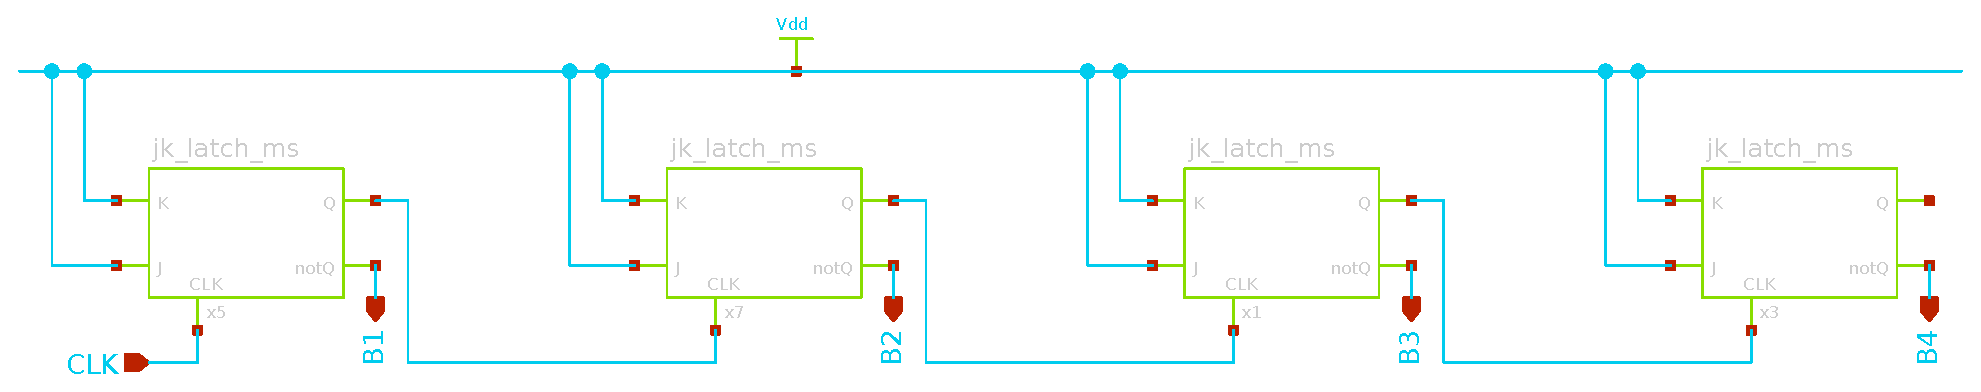
\includegraphics[width=\linewidth]{Immagini/count-sch}
		\caption{schema a blocchi di un contatore binario con risoluzione a 4 bit.}
		\label{fig:count:sch}
	\end{figure}
	
	Facendo riferimento al contatore binario in figura \ref{fig:count:sch}, si osserva che $B_1$ è il bit meno significativo, mentre $B_4$ è il bit più significativo.
	
	Va inoltre rilevato che l'uscita del segnale $Q$ viene immessa come segnale di clock nel flip-flop JK seguente, mentre l'uscita che misura il valore in uscita è rilevata dall'uscita negata $\overline Q$: questo è dovuto al fatto che l'interconnessione così implementata genera dei fronti di salita complementari al valore effettivo. Supponendo infatti che all'istante iniziale tutte le uscite $Q$ dei flip-flop siano poste allo stato logico basso, al primo ingresso di clock tutte commuterebbero, per via di una reazione a cascata, allo stato logico alto. L'effetto che si osserva dal circuito è dunque quello di contatore inverso (che dal valore massimo scorre al valore minimo), tuttavia leggendo le uscite negate $\overline Q$ si torna a leggere il conteggio in modo corretto.
	
	\begin{figure}[bht]
		\centering
		% GNUPLOT: LaTeX picture with Postscript
\begingroup
  \makeatletter
  \providecommand\color[2][]{%
    \GenericError{(gnuplot) \space\space\space\@spaces}{%
      Package color not loaded in conjunction with
      terminal option `colourtext'%
    }{See the gnuplot documentation for explanation.%
    }{Either use 'blacktext' in gnuplot or load the package
      color.sty in LaTeX.}%
    \renewcommand\color[2][]{}%
  }%
  \providecommand\includegraphics[2][]{%
    \GenericError{(gnuplot) \space\space\space\@spaces}{%
      Package graphicx or graphics not loaded%
    }{See the gnuplot documentation for explanation.%
    }{The gnuplot epslatex terminal needs graphicx.sty or graphics.sty.}%
    \renewcommand\includegraphics[2][]{}%
  }%
  \providecommand\rotatebox[2]{#2}%
  \@ifundefined{ifGPcolor}{%
    \newif\ifGPcolor
    \GPcolorfalse
  }{}%
  \@ifundefined{ifGPblacktext}{%
    \newif\ifGPblacktext
    \GPblacktexttrue
  }{}%
  % define a \g@addto@macro without @ in the name:
  \let\gplgaddtomacro\g@addto@macro
  % define empty templates for all commands taking text:
  \gdef\gplbacktext{}%
  \gdef\gplfronttext{}%
  \makeatother
  \ifGPblacktext
    % no textcolor at all
    \def\colorrgb#1{}%
    \def\colorgray#1{}%
  \else
    % gray or color?
    \ifGPcolor
      \def\colorrgb#1{\color[rgb]{#1}}%
      \def\colorgray#1{\color[gray]{#1}}%
      \expandafter\def\csname LTw\endcsname{\color{white}}%
      \expandafter\def\csname LTb\endcsname{\color{black}}%
      \expandafter\def\csname LTa\endcsname{\color{black}}%
      \expandafter\def\csname LT0\endcsname{\color[rgb]{1,0,0}}%
      \expandafter\def\csname LT1\endcsname{\color[rgb]{0,1,0}}%
      \expandafter\def\csname LT2\endcsname{\color[rgb]{0,0,1}}%
      \expandafter\def\csname LT3\endcsname{\color[rgb]{1,0,1}}%
      \expandafter\def\csname LT4\endcsname{\color[rgb]{0,1,1}}%
      \expandafter\def\csname LT5\endcsname{\color[rgb]{1,1,0}}%
      \expandafter\def\csname LT6\endcsname{\color[rgb]{0,0,0}}%
      \expandafter\def\csname LT7\endcsname{\color[rgb]{1,0.3,0}}%
      \expandafter\def\csname LT8\endcsname{\color[rgb]{0.5,0.5,0.5}}%
    \else
      % gray
      \def\colorrgb#1{\color{black}}%
      \def\colorgray#1{\color[gray]{#1}}%
      \expandafter\def\csname LTw\endcsname{\color{white}}%
      \expandafter\def\csname LTb\endcsname{\color{black}}%
      \expandafter\def\csname LTa\endcsname{\color{black}}%
      \expandafter\def\csname LT0\endcsname{\color{black}}%
      \expandafter\def\csname LT1\endcsname{\color{black}}%
      \expandafter\def\csname LT2\endcsname{\color{black}}%
      \expandafter\def\csname LT3\endcsname{\color{black}}%
      \expandafter\def\csname LT4\endcsname{\color{black}}%
      \expandafter\def\csname LT5\endcsname{\color{black}}%
      \expandafter\def\csname LT6\endcsname{\color{black}}%
      \expandafter\def\csname LT7\endcsname{\color{black}}%
      \expandafter\def\csname LT8\endcsname{\color{black}}%
    \fi
  \fi
    \setlength{\unitlength}{0.0500bp}%
    \ifx\gptboxheight\undefined%
      \newlength{\gptboxheight}%
      \newlength{\gptboxwidth}%
      \newsavebox{\gptboxtext}%
    \fi%
    \setlength{\fboxrule}{0.5pt}%
    \setlength{\fboxsep}{1pt}%
\begin{picture}(5668.00,4534.00)%
    \gplgaddtomacro\gplbacktext{%
      \csname LTb\endcsname%%
      \put(434,3795){\makebox(0,0)[r]{\strut{}$0$}}%
      \csname LTb\endcsname%%
      \put(434,4107){\makebox(0,0)[r]{\strut{}$0.9$}}%
      \csname LTb\endcsname%%
      \put(434,4418){\makebox(0,0)[r]{\strut{}$1.8$}}%
      \csname LTb\endcsname%%
      \put(566,3506){\makebox(0,0){\strut{}}}%
      \csname LTb\endcsname%%
      \put(1770,3506){\makebox(0,0){\strut{}}}%
      \csname LTb\endcsname%%
      \put(2975,3506){\makebox(0,0){\strut{}}}%
      \csname LTb\endcsname%%
      \put(4179,3506){\makebox(0,0){\strut{}}}%
      \csname LTb\endcsname%%
      \put(5383,3506){\makebox(0,0){\strut{}}}%
    }%
    \gplgaddtomacro\gplfronttext{%
      \csname LTb\endcsname%%
      \put(-171,4106){\rotatebox{-270}{\makebox(0,0){\strut{}$B_4$}}}%
      \put(2974,3440){\makebox(0,0){\strut{}}}%
    }%
    \gplgaddtomacro\gplbacktext{%
      \csname LTb\endcsname%%
      \put(434,3034){\makebox(0,0)[r]{\strut{}$0$}}%
      \csname LTb\endcsname%%
      \put(434,3346){\makebox(0,0)[r]{\strut{}$0.9$}}%
      \csname LTb\endcsname%%
      \put(434,3657){\makebox(0,0)[r]{\strut{}$1.8$}}%
      \csname LTb\endcsname%%
      \put(566,2745){\makebox(0,0){\strut{}}}%
      \csname LTb\endcsname%%
      \put(1770,2745){\makebox(0,0){\strut{}}}%
      \csname LTb\endcsname%%
      \put(2975,2745){\makebox(0,0){\strut{}}}%
      \csname LTb\endcsname%%
      \put(4179,2745){\makebox(0,0){\strut{}}}%
      \csname LTb\endcsname%%
      \put(5383,2745){\makebox(0,0){\strut{}}}%
    }%
    \gplgaddtomacro\gplfronttext{%
      \csname LTb\endcsname%%
      \put(-171,3345){\rotatebox{-270}{\makebox(0,0){\strut{}$B_3$}}}%
      \put(2974,2679){\makebox(0,0){\strut{}}}%
    }%
    \gplgaddtomacro\gplbacktext{%
      \csname LTb\endcsname%%
      \put(434,2272){\makebox(0,0)[r]{\strut{}$0$}}%
      \csname LTb\endcsname%%
      \put(434,2584){\makebox(0,0)[r]{\strut{}$0.9$}}%
      \csname LTb\endcsname%%
      \put(434,2895){\makebox(0,0)[r]{\strut{}$1.8$}}%
      \csname LTb\endcsname%%
      \put(566,1983){\makebox(0,0){\strut{}}}%
      \csname LTb\endcsname%%
      \put(1770,1983){\makebox(0,0){\strut{}}}%
      \csname LTb\endcsname%%
      \put(2975,1983){\makebox(0,0){\strut{}}}%
      \csname LTb\endcsname%%
      \put(4179,1983){\makebox(0,0){\strut{}}}%
      \csname LTb\endcsname%%
      \put(5383,1983){\makebox(0,0){\strut{}}}%
    }%
    \gplgaddtomacro\gplfronttext{%
      \csname LTb\endcsname%%
      \put(-171,2583){\rotatebox{-270}{\makebox(0,0){\strut{}$B_2$}}}%
      \put(2974,1917){\makebox(0,0){\strut{}}}%
    }%
    \gplgaddtomacro\gplbacktext{%
      \csname LTb\endcsname%%
      \put(434,1510){\makebox(0,0)[r]{\strut{}$0$}}%
      \csname LTb\endcsname%%
      \put(434,1822){\makebox(0,0)[r]{\strut{}$0.9$}}%
      \csname LTb\endcsname%%
      \put(434,2134){\makebox(0,0)[r]{\strut{}$1.8$}}%
      \csname LTb\endcsname%%
      \put(566,1221){\makebox(0,0){\strut{}}}%
      \csname LTb\endcsname%%
      \put(1770,1221){\makebox(0,0){\strut{}}}%
      \csname LTb\endcsname%%
      \put(2975,1221){\makebox(0,0){\strut{}}}%
      \csname LTb\endcsname%%
      \put(4179,1221){\makebox(0,0){\strut{}}}%
      \csname LTb\endcsname%%
      \put(5383,1221){\makebox(0,0){\strut{}}}%
    }%
    \gplgaddtomacro\gplfronttext{%
      \csname LTb\endcsname%%
      \put(-171,1822){\rotatebox{-270}{\makebox(0,0){\strut{}$B_1$}}}%
      \put(2974,1155){\makebox(0,0){\strut{}}}%
    }%
    \gplgaddtomacro\gplbacktext{%
      \csname LTb\endcsname%%
      \put(434,749){\makebox(0,0)[r]{\strut{}$0$}}%
      \csname LTb\endcsname%%
      \put(434,1061){\makebox(0,0)[r]{\strut{}$0.9$}}%
      \csname LTb\endcsname%%
      \put(434,1372){\makebox(0,0)[r]{\strut{}$1.8$}}%
      \csname LTb\endcsname%%
      \put(566,460){\makebox(0,0){\strut{}0}}%
      \csname LTb\endcsname%%
      \put(1770,460){\makebox(0,0){\strut{}0.5}}%
      \csname LTb\endcsname%%
      \put(2975,460){\makebox(0,0){\strut{}1}}%
      \csname LTb\endcsname%%
      \put(4179,460){\makebox(0,0){\strut{}1.5}}%
      \csname LTb\endcsname%%
      \put(5383,460){\makebox(0,0){\strut{}2}}%
    }%
    \gplgaddtomacro\gplfronttext{%
      \csname LTb\endcsname%%
      \put(-171,1060){\rotatebox{-270}{\makebox(0,0){\strut{}$CLK$}}}%
      \put(2974,130){\makebox(0,0){\strut{}tempo $[\mu s]$}}%
    }%
    \gplbacktext
    \put(0,0){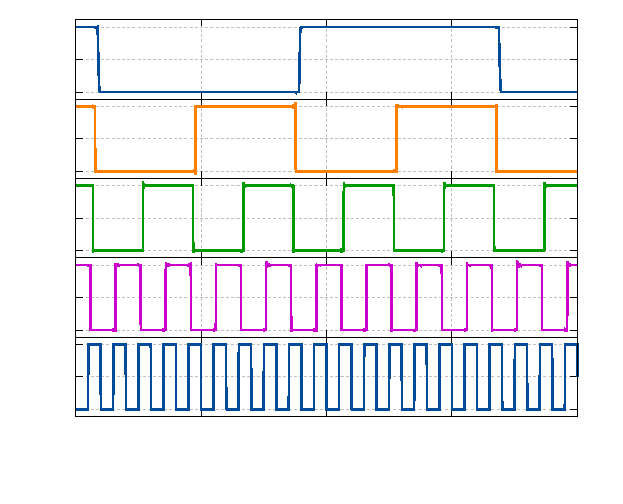
\includegraphics[width={283.40bp},height={226.70bp}]{Immagini/count-mult}}%
    \gplfronttext
  \end{picture}%
\endgroup


		\vspace{3mm}
		\caption{andamento in funzione del tempo del valore dei bit rilevati dal contatore binario a 4 bit (figura \ref{fig:count:sch}) in funzione del segnale di clock $CLK$. Le uscite del circuito sono poste a massa tramite una capacità di carico di $0.75pF$. Le tensioni sono espresse in volt.}
		\label{fig:count:mult}
	\end{figure}
	
	Tramite una simulazione nel dominio del tempo, il cui risultato è raffigurato in figura \ref{fig:count:mult}, è possibile osservare il corretto funzionamento del circuito. Considerando per esempio di voler calcolare il numero di fronti di salita del segnale di clock al tempo $t=1.5\mu s$ è sufficiente analizzare i singoli bit: $B_1 = 0$, $B_2 = 1$, $B_3=1$ e $B_4=1$. Componendo il numero binario è possibile anche effettuare la conversione in decimale:
	\[ 1110_2 = 14_{10} \]
	Contando il numero di clock effettivamente trascorsi, si osserva che essi sono 15, tuttavia il primo di questi impulsi (per via delle condizioni iniziali del circuito) serve a impostare a 0 tutti bit del circuito, e dunque non viene conteggiato dal contatore binario.
	
	Da questo circuito è possibile ricavare delle soluzioni più complesse che permettano di azzerare il conteggio oppure di abilitare (o meno) la lettura del segnale di clock, in quanto tali funzionalità (allo stato di implementazione attuale) non possono essere effettuate.
	
\subsection*{Contatore con segnale di reset e di enable}
	
	Sfruttando il circuito appena descritto per effettuare il conteggio binario mediante la rilevazione di impulsi di clock, è possibile aggiungere delle funzionalità allo stesso mediante l'aggiunta di altri segnali e porte logiche. 
	
	\begin{figure}[bht]
		\centering
		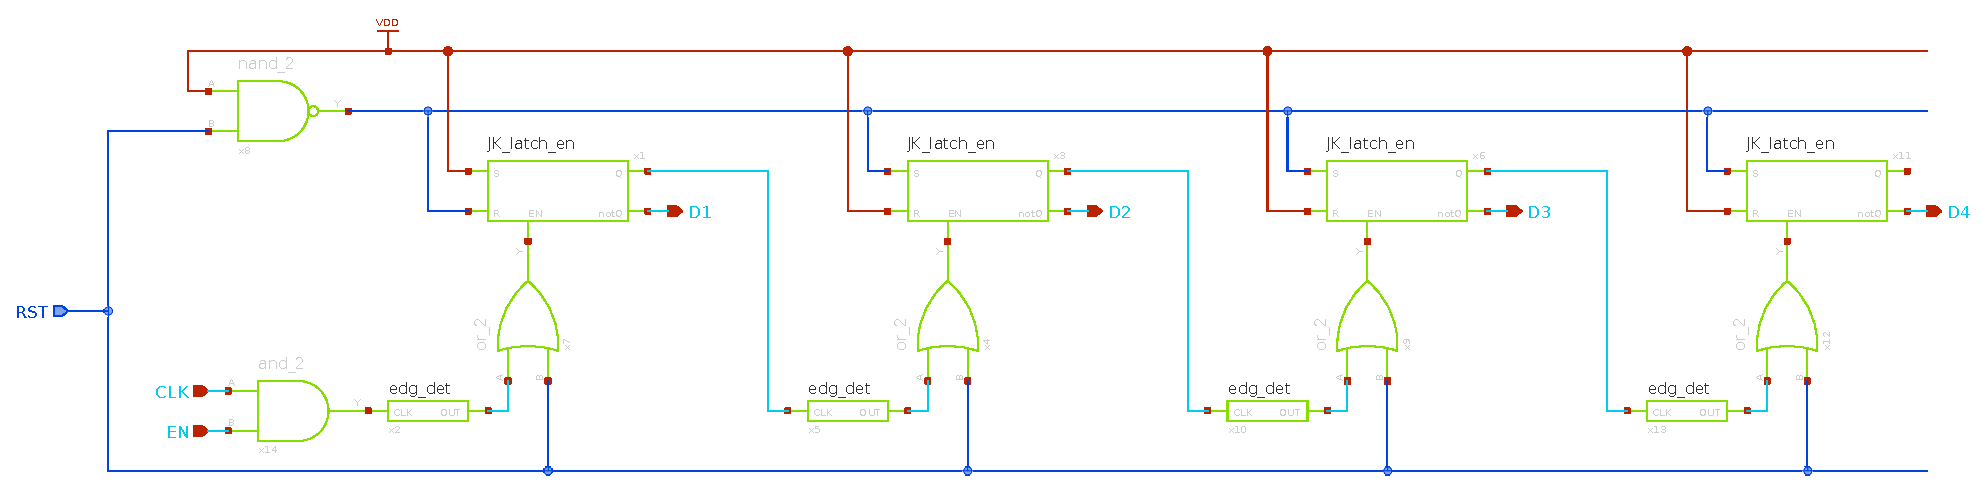
\includegraphics[width=\linewidth]{Immagini/count2-sch}
		\caption{schematico di un contatore binario con risoluzione a 4 bit con segnale di reset e di abilitazione al conteggio.}
		\label{fig:count:resen}
	\end{figure}
	
	In figura \ref{fig:count:resen} è mostrata un'implementazione circuitale di un contatore binario al quale sono state aggiunte le funzionalità di reset (segnale $RST$) e di abilitazione al conteggio (segnale $EN$). Per realizzare questo tipo di circuito è stato necessario separare il circuito di edge detection del flip-flop JK master-slave dal latch JK vero e proprio. 
	
	\paragraph{Funzione di abilitazione} La funzione di abilitazione del conteggio è semplice da realizzare, e si basa sul filtrare il segnale di clock in ingresso mediante una porta logica and il cui secondo input è il segnale di abilitazione. Quando $EN$ si trova allo stato alto allora gli impulsi di clock potranno essere correttamente inviati al circuito di edge detection, mentre se $EN$ fosse basso nessun impulso verrebbe mandato come ingresso al contatore.
	
	\paragraph{Funzione di reset} La funzione di reset è più complessa ed è costituita dalle connessioni in blu in figura \ref{fig:count:resen}. Tale comportamento desiderato è ottenuto mediante due passaggi: quando il segnale di reset assume uno stato logico alto tutti i latch vengono resettati (tranne il primo latch che per riuscire a rilevare correttamente il primo impulso deve essere impostato per avere un'uscita alta) mediante il gate nand (sfruttandone la sua tabella di verità) i cui ingressi sono il segnale $RST$ e la tensione di alimentazione.\\
	Il secondo step è quello di abilitare gli ingressi di tutti i latch JK: in questo modo ogni primo stadio dei latch del contatore verrà inizializzato al valore iniziale prestabilito. Nell'immeddiato l'uscita di reset non risulta evidente, tuttavia appena il segnale $RST$ torna allo stato logico basso il latch master invierà il segnale allo slave effettuando di fatto il ripristino ad uno stato noto del circuito.
	
	
	\begin{figure}[p]
		\centering
		% GNUPLOT: LaTeX picture with Postscript
\begingroup
  \makeatletter
  \providecommand\color[2][]{%
    \GenericError{(gnuplot) \space\space\space\@spaces}{%
      Package color not loaded in conjunction with
      terminal option `colourtext'%
    }{See the gnuplot documentation for explanation.%
    }{Either use 'blacktext' in gnuplot or load the package
      color.sty in LaTeX.}%
    \renewcommand\color[2][]{}%
  }%
  \providecommand\includegraphics[2][]{%
    \GenericError{(gnuplot) \space\space\space\@spaces}{%
      Package graphicx or graphics not loaded%
    }{See the gnuplot documentation for explanation.%
    }{The gnuplot epslatex terminal needs graphicx.sty or graphics.sty.}%
    \renewcommand\includegraphics[2][]{}%
  }%
  \providecommand\rotatebox[2]{#2}%
  \@ifundefined{ifGPcolor}{%
    \newif\ifGPcolor
    \GPcolorfalse
  }{}%
  \@ifundefined{ifGPblacktext}{%
    \newif\ifGPblacktext
    \GPblacktexttrue
  }{}%
  % define a \g@addto@macro without @ in the name:
  \let\gplgaddtomacro\g@addto@macro
  % define empty templates for all commands taking text:
  \gdef\gplbacktext{}%
  \gdef\gplfronttext{}%
  \makeatother
  \ifGPblacktext
    % no textcolor at all
    \def\colorrgb#1{}%
    \def\colorgray#1{}%
  \else
    % gray or color?
    \ifGPcolor
      \def\colorrgb#1{\color[rgb]{#1}}%
      \def\colorgray#1{\color[gray]{#1}}%
      \expandafter\def\csname LTw\endcsname{\color{white}}%
      \expandafter\def\csname LTb\endcsname{\color{black}}%
      \expandafter\def\csname LTa\endcsname{\color{black}}%
      \expandafter\def\csname LT0\endcsname{\color[rgb]{1,0,0}}%
      \expandafter\def\csname LT1\endcsname{\color[rgb]{0,1,0}}%
      \expandafter\def\csname LT2\endcsname{\color[rgb]{0,0,1}}%
      \expandafter\def\csname LT3\endcsname{\color[rgb]{1,0,1}}%
      \expandafter\def\csname LT4\endcsname{\color[rgb]{0,1,1}}%
      \expandafter\def\csname LT5\endcsname{\color[rgb]{1,1,0}}%
      \expandafter\def\csname LT6\endcsname{\color[rgb]{0,0,0}}%
      \expandafter\def\csname LT7\endcsname{\color[rgb]{1,0.3,0}}%
      \expandafter\def\csname LT8\endcsname{\color[rgb]{0.5,0.5,0.5}}%
    \else
      % gray
      \def\colorrgb#1{\color{black}}%
      \def\colorgray#1{\color[gray]{#1}}%
      \expandafter\def\csname LTw\endcsname{\color{white}}%
      \expandafter\def\csname LTb\endcsname{\color{black}}%
      \expandafter\def\csname LTa\endcsname{\color{black}}%
      \expandafter\def\csname LT0\endcsname{\color{black}}%
      \expandafter\def\csname LT1\endcsname{\color{black}}%
      \expandafter\def\csname LT2\endcsname{\color{black}}%
      \expandafter\def\csname LT3\endcsname{\color{black}}%
      \expandafter\def\csname LT4\endcsname{\color{black}}%
      \expandafter\def\csname LT5\endcsname{\color{black}}%
      \expandafter\def\csname LT6\endcsname{\color{black}}%
      \expandafter\def\csname LT7\endcsname{\color{black}}%
      \expandafter\def\csname LT8\endcsname{\color{black}}%
    \fi
  \fi
    \setlength{\unitlength}{0.0500bp}%
    \ifx\gptboxheight\undefined%
      \newlength{\gptboxheight}%
      \newlength{\gptboxwidth}%
      \newsavebox{\gptboxtext}%
    \fi%
    \setlength{\fboxrule}{0.5pt}%
    \setlength{\fboxsep}{1pt}%
\begin{picture}(6802.00,7652.00)%
    \gplgaddtomacro\gplbacktext{%
      \csname LTb\endcsname%%
      \put(548,6740){\makebox(0,0)[r]{\strut{}$0$}}%
      \csname LTb\endcsname%%
      \put(548,7116){\makebox(0,0)[r]{\strut{}$0.9$}}%
      \csname LTb\endcsname%%
      \put(548,7491){\makebox(0,0)[r]{\strut{}$1.8$}}%
      \csname LTb\endcsname%%
      \put(680,6437){\makebox(0,0){\strut{}}}%
      \csname LTb\endcsname%%
      \put(2125,6437){\makebox(0,0){\strut{}}}%
      \csname LTb\endcsname%%
      \put(3570,6437){\makebox(0,0){\strut{}}}%
      \csname LTb\endcsname%%
      \put(5015,6437){\makebox(0,0){\strut{}}}%
      \csname LTb\endcsname%%
      \put(6460,6437){\makebox(0,0){\strut{}}}%
    }%
    \gplgaddtomacro\gplfronttext{%
      \csname LTb\endcsname%%
      \put(-57,7115){\rotatebox{-270}{\makebox(0,0){\strut{}$D_4$}}}%
      \put(3570,6371){\makebox(0,0){\strut{}}}%
    }%
    \gplgaddtomacro\gplbacktext{%
      \csname LTb\endcsname%%
      \put(548,5822){\makebox(0,0)[r]{\strut{}$0$}}%
      \csname LTb\endcsname%%
      \put(548,6198){\makebox(0,0)[r]{\strut{}$0.9$}}%
      \csname LTb\endcsname%%
      \put(548,6573){\makebox(0,0)[r]{\strut{}$1.8$}}%
      \csname LTb\endcsname%%
      \put(680,5519){\makebox(0,0){\strut{}}}%
      \csname LTb\endcsname%%
      \put(2125,5519){\makebox(0,0){\strut{}}}%
      \csname LTb\endcsname%%
      \put(3570,5519){\makebox(0,0){\strut{}}}%
      \csname LTb\endcsname%%
      \put(5015,5519){\makebox(0,0){\strut{}}}%
      \csname LTb\endcsname%%
      \put(6460,5519){\makebox(0,0){\strut{}}}%
    }%
    \gplgaddtomacro\gplfronttext{%
      \csname LTb\endcsname%%
      \put(-57,6197){\rotatebox{-270}{\makebox(0,0){\strut{}$D_3$}}}%
      \put(3570,5453){\makebox(0,0){\strut{}}}%
    }%
    \gplgaddtomacro\gplbacktext{%
      \csname LTb\endcsname%%
      \put(548,4903){\makebox(0,0)[r]{\strut{}$0$}}%
      \csname LTb\endcsname%%
      \put(548,5279){\makebox(0,0)[r]{\strut{}$0.9$}}%
      \csname LTb\endcsname%%
      \put(548,5655){\makebox(0,0)[r]{\strut{}$1.8$}}%
      \csname LTb\endcsname%%
      \put(680,4600){\makebox(0,0){\strut{}}}%
      \csname LTb\endcsname%%
      \put(2125,4600){\makebox(0,0){\strut{}}}%
      \csname LTb\endcsname%%
      \put(3570,4600){\makebox(0,0){\strut{}}}%
      \csname LTb\endcsname%%
      \put(5015,4600){\makebox(0,0){\strut{}}}%
      \csname LTb\endcsname%%
      \put(6460,4600){\makebox(0,0){\strut{}}}%
    }%
    \gplgaddtomacro\gplfronttext{%
      \csname LTb\endcsname%%
      \put(-57,5279){\rotatebox{-270}{\makebox(0,0){\strut{}$D_2$}}}%
      \put(3570,4534){\makebox(0,0){\strut{}}}%
    }%
    \gplgaddtomacro\gplbacktext{%
      \csname LTb\endcsname%%
      \put(548,3985){\makebox(0,0)[r]{\strut{}$0$}}%
      \csname LTb\endcsname%%
      \put(548,4361){\makebox(0,0)[r]{\strut{}$0.9$}}%
      \csname LTb\endcsname%%
      \put(548,4737){\makebox(0,0)[r]{\strut{}$1.8$}}%
      \csname LTb\endcsname%%
      \put(680,3682){\makebox(0,0){\strut{}}}%
      \csname LTb\endcsname%%
      \put(2125,3682){\makebox(0,0){\strut{}}}%
      \csname LTb\endcsname%%
      \put(3570,3682){\makebox(0,0){\strut{}}}%
      \csname LTb\endcsname%%
      \put(5015,3682){\makebox(0,0){\strut{}}}%
      \csname LTb\endcsname%%
      \put(6460,3682){\makebox(0,0){\strut{}}}%
    }%
    \gplgaddtomacro\gplfronttext{%
      \csname LTb\endcsname%%
      \put(-57,4361){\rotatebox{-270}{\makebox(0,0){\strut{}$D_1$}}}%
      \put(3570,3616){\makebox(0,0){\strut{}}}%
    }%
    \gplgaddtomacro\gplbacktext{%
      \csname LTb\endcsname%%
      \put(548,3067){\makebox(0,0)[r]{\strut{}$0$}}%
      \csname LTb\endcsname%%
      \put(548,3443){\makebox(0,0)[r]{\strut{}$0.9$}}%
      \csname LTb\endcsname%%
      \put(548,3819){\makebox(0,0)[r]{\strut{}$1.8$}}%
      \csname LTb\endcsname%%
      \put(680,2764){\makebox(0,0){\strut{}}}%
      \csname LTb\endcsname%%
      \put(2125,2764){\makebox(0,0){\strut{}}}%
      \csname LTb\endcsname%%
      \put(3570,2764){\makebox(0,0){\strut{}}}%
      \csname LTb\endcsname%%
      \put(5015,2764){\makebox(0,0){\strut{}}}%
      \csname LTb\endcsname%%
      \put(6460,2764){\makebox(0,0){\strut{}}}%
    }%
    \gplgaddtomacro\gplfronttext{%
      \csname LTb\endcsname%%
      \put(-57,3443){\rotatebox{-270}{\makebox(0,0){\strut{}$EN$}}}%
      \put(3570,2698){\makebox(0,0){\strut{}}}%
    }%
    \gplgaddtomacro\gplbacktext{%
      \csname LTb\endcsname%%
      \put(548,2149){\makebox(0,0)[r]{\strut{}$0$}}%
      \csname LTb\endcsname%%
      \put(548,2525){\makebox(0,0)[r]{\strut{}$0.9$}}%
      \csname LTb\endcsname%%
      \put(548,2900){\makebox(0,0)[r]{\strut{}$1.8$}}%
      \csname LTb\endcsname%%
      \put(680,1846){\makebox(0,0){\strut{}}}%
      \csname LTb\endcsname%%
      \put(2125,1846){\makebox(0,0){\strut{}}}%
      \csname LTb\endcsname%%
      \put(3570,1846){\makebox(0,0){\strut{}}}%
      \csname LTb\endcsname%%
      \put(5015,1846){\makebox(0,0){\strut{}}}%
      \csname LTb\endcsname%%
      \put(6460,1846){\makebox(0,0){\strut{}}}%
    }%
    \gplgaddtomacro\gplfronttext{%
      \csname LTb\endcsname%%
      \put(-57,2524){\rotatebox{-270}{\makebox(0,0){\strut{}$RST$}}}%
      \put(3570,1780){\makebox(0,0){\strut{}}}%
    }%
    \gplgaddtomacro\gplbacktext{%
      \csname LTb\endcsname%%
      \put(548,1230){\makebox(0,0)[r]{\strut{}$0$}}%
      \csname LTb\endcsname%%
      \put(548,1606){\makebox(0,0)[r]{\strut{}$0.9$}}%
      \csname LTb\endcsname%%
      \put(548,1982){\makebox(0,0)[r]{\strut{}$1.8$}}%
      \csname LTb\endcsname%%
      \put(680,927){\makebox(0,0){\strut{}0}}%
      \csname LTb\endcsname%%
      \put(2125,927){\makebox(0,0){\strut{}500}}%
      \csname LTb\endcsname%%
      \put(3570,927){\makebox(0,0){\strut{}1000}}%
      \csname LTb\endcsname%%
      \put(5015,927){\makebox(0,0){\strut{}1500}}%
      \csname LTb\endcsname%%
      \put(6460,927){\makebox(0,0){\strut{}2000}}%
    }%
    \gplgaddtomacro\gplfronttext{%
      \csname LTb\endcsname%%
      \put(-57,1606){\rotatebox{-270}{\makebox(0,0){\strut{}$CLK$}}}%
      \put(3570,597){\makebox(0,0){\strut{}tempo $[ns]$}}%
    }%
    \gplbacktext
    \put(0,0){\includegraphics[width={340.10bp},height={382.60bp}]{Immagini/counter-improved}}%
    \gplfronttext
  \end{picture}%
\endgroup



		\vspace{4mm}
		\caption{andamento in funzione del tempo dei bit di un contatore binario a 4 bit (figura \ref{fig:count:resen}) in funzione del segnale di clock $CLK$, di abilitazione $EN$ e reset $RST$. Ogni uscita del circuito è collegata a massa mediante una capacità di carico di $0.75pF$. Le tensioni sono espresse in volt.  }
		\label{fig:count:simresen}
	\end{figure}

	\paragraph{Simulazione} Nella pagina seguente, in figura \ref{fig:count:simresen}, è possibile osservare una simulazione nel dominio del tempo del circuito, osservando come le uscite rispettino le condizione di reset imposte dal relativo segnale e l'abilitazione permetta (o meno) il conteggio degli impulsi di clock.
	
\section{Sommatore binario}
\subsection*{Half adder}
	Un circuito che permette di effettuare la somma binaria di due numeri è composto da una serie di moduli elementari che permettono di effettuare la somma bit-a-bit. Per questo è importante studiare le varianti di questa sezioni circuitali per comprendere il funzionamento del circuito che dovranno comporre.
	
	Il primo elemento che si può studiare è l'\textit{half adder} (mezzo sommatore), un elemento che viene utilizzato per determinare la somma di due bit. Tale circuito deve dunque prevedere necessariamente due ingressi $A$ e $B$, associati ai valori logici da sommare, mentre le uscite sono 2: il risultato $R$ della somma binaria e l'eventuale riporto $C$ (dall'inglese \textit{carry}).
	
	La somma di due bit in un sistema binario può essere velocemente analizzata tramite la realizzazione della tabella di verità \ref{tab:ha:tabella}, dove la terza colonna $R_{10}$ rappresenta il risultato in cifra decimale.
	
	\begin{table}[bht]
		\centering
		\begin{tabular}{c c | c | c c }
			$A$ & $B$ & $R_{10}$ & $C$ & $R$ \\ \hline
			0 & 0 & 0 & 0 & 0 \\	
			0 & 1 & 1 & 0 & 1 \\	
			1 & 0 & 1 & 0 & 1 \\
			1 & 1 & 2 & 1 & 0 \\		
		\end{tabular}
		\caption{tabella di verità associata alla somma di due bit $A$ e $B$. La colonna $R_{10}$ rappresenta il risultato della somma binaria espressa come cifra decimale. Il risultato della somma può essere letto digitalmente concatenando il carry $C$ con il risultato $R$.}
		\label{tab:ha:tabella}
	\end{table}
	
	Dalla tabella di verità che deve essere verificata dal circuito del mezzo sommatore è evidente osservare come il carry $C$ sia determinato dal prodotto logico degli ingressi binari, mentre $R$ sia ottenuto come or esclusivo degli stessi. Questo permette di implementare circuitalmente le porte logiche come in figura \ref{fig:ha:sch}.
	
	\begin{figure}[H]
		\centering
		\begin{subfigure}{0.48\linewidth}
			\centering
			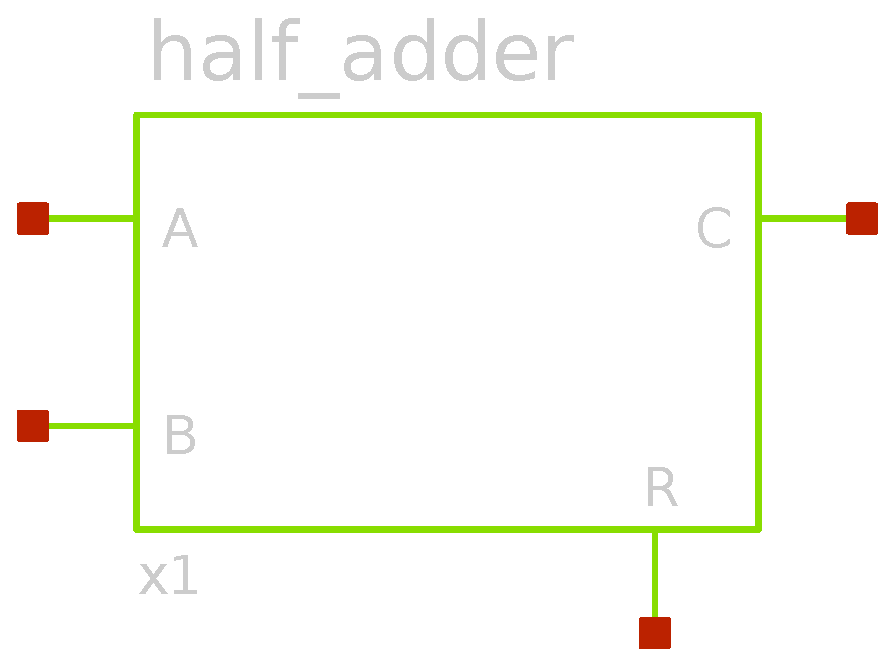
\includegraphics[width=3cm]{Immagini/half-adder}
			\caption{}
		\end{subfigure}
		\begin{subfigure}{0.48\linewidth}
			\centering
			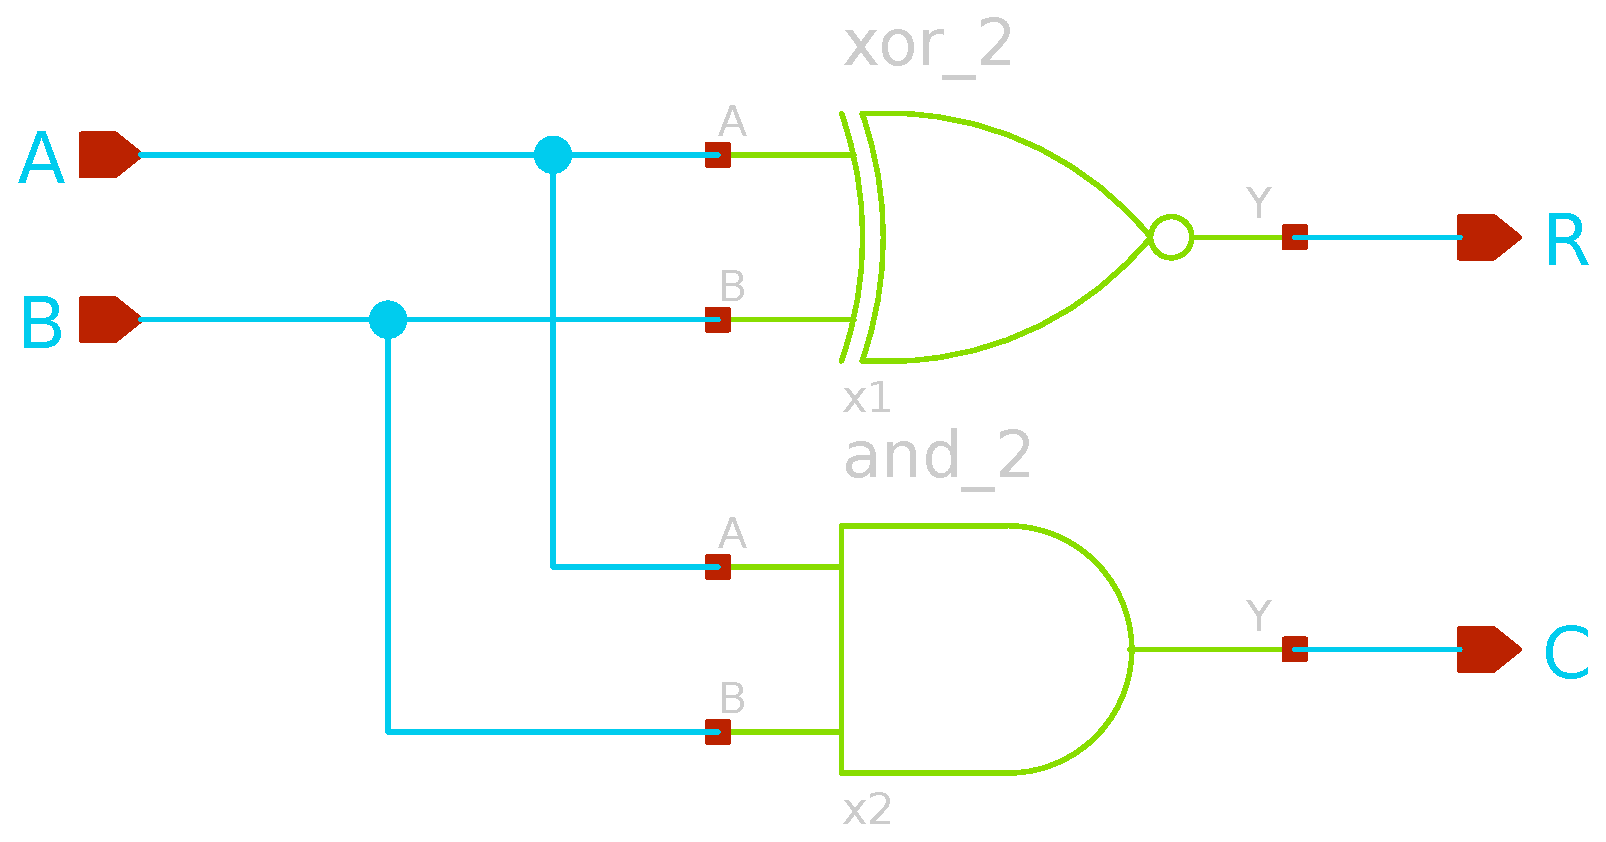
\includegraphics[width=5cm]{Immagini/half-adder-sch}
			\caption{}
		\end{subfigure}
		\caption{rappresentazione simbolica del blocco half adder (a) e relativa implementazione mediante gate logici (b).}
		\label{fig:ha:sch}
	\end{figure}
	
	Il corretto funzionamento del circuito mezzo sommatore può essere verificato anche mediante una simulazione nel dominio del tempo i cui risultati sono mostrati in figura \ref{fig:ha:sim}.	
	\begin{figure}[bht]
		\centering
		\input{Immagini/half-adder-sim}
		\caption{risposta nel dominio del tempo delle uscite dell'half adder in funzione delle possibili combinazioni d'ingresso. Le uscite del circuito sono collegate a massa mediante una capacità di carico di $0.75pf$. Le tensioni sono misurate in volt.}
		\label{fig:ha:sim}
	\end{figure}

\subsection*{Full adder}
	Il mezzo sommatore appena descritto è funzionante rispetto alla somma binaria, tuttavia presenta delle limitazioni che ne impediscono l'utilizzo pratico. Infatti questo circuito non permette di considerare un eventuale riporto dovuto ad un sommatore posto a monte.
	
	Per ovviare a questo problema è possibile costruire il \textit{full adder}, ossia un circuito che è in grado di effettuare la somma di due bit $A$ e $B$ considerando anche l'eventuale riporto in ingresso $C_{in}$ da un sommatore a monte. Le uscite, in analogia al mezzo sommatore, sono il risultato $R$ dell'operazione di somma bit-a-bit e il riporto in uscita $C_{out}$.
	
	Anche in questo caso è possibile realizzare il circuito del full adder mediante previa costruzione della tabella di verità \ref{tab:fa:tabella}.
	
	
	\begin{table}[bht]
		\centering
		\begin{tabular}{c c c | c | c c }
			$A$ & $B$ & $C_{in}$ & $R_{10}$ & $C_{out}$ & $R$ \\ \hline
			0 & 0 & 0 & 0 & 0 & 0 \\	
			0 & 1 & 0 & 1 & 0 & 1 \\	
			1 & 0 & 0 & 1 & 0 & 1 \\
			1 & 1 & 0 & 2 & 1 & 0 \\
			0 & 0 & 1 & 1 & 0 & 1 \\	
			0 & 1 & 1 & 2 & 1 & 0 \\	
			1 & 0 & 1 & 2 & 1 & 0 \\
			1 & 1 & 1 & 3 & 1 & 1 \\				
		\end{tabular}
		\caption{tabella di verità di un full adder associata alla somma di due bit $A$ e $B$ con riporto in ingresso $C_{in}$. La colonna $R_{10}$ rappresenta il risultato della somma binaria espressa come cifra decimale. Il risultato della somma può essere letto digitalmente concatenando il riporto in uscita $C_{out}$ con il risultato $R$.}
		\label{tab:fa:tabella}
	\end{table}
	
	A questo punto è possibile costruire un circuito, mediante l'utilizzo di porte logiche, in grado di realizzare tale tabella di verità la cui implementazione logica è mostrata in figura \ref{fig:fa:sch} e rispetto ad essa è possibile trarre delle conclusioni sul funzionamento del circuito.
	
	\begin{figure}[bht]
		\centering
		\begin{subfigure}{0.48\linewidth}
			\centering
			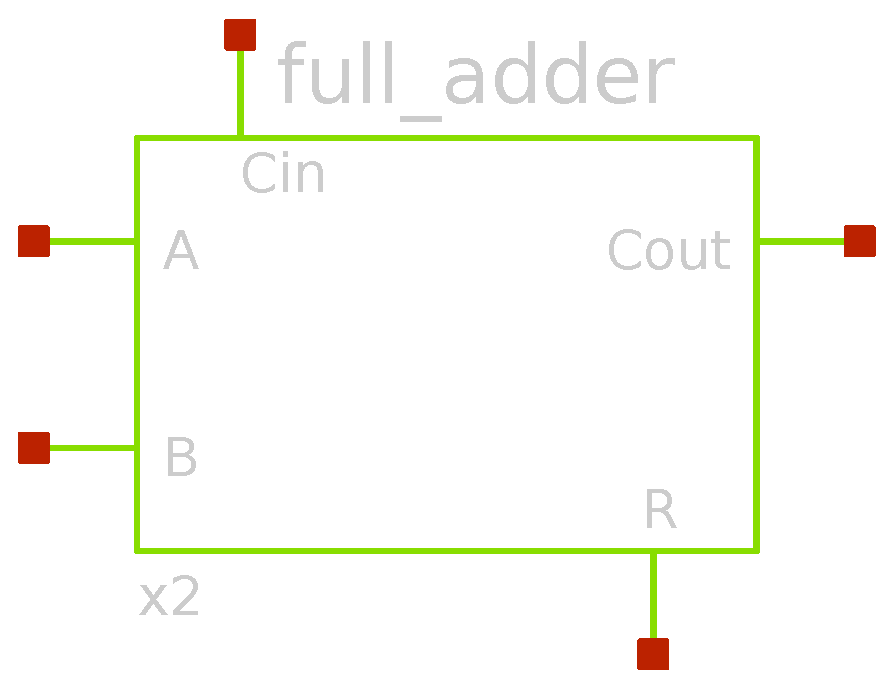
\includegraphics[width=3cm]{Immagini/full-adder-sch}
			\caption{}
		\end{subfigure}
		\begin{subfigure}{0.48\linewidth}
			\centering
			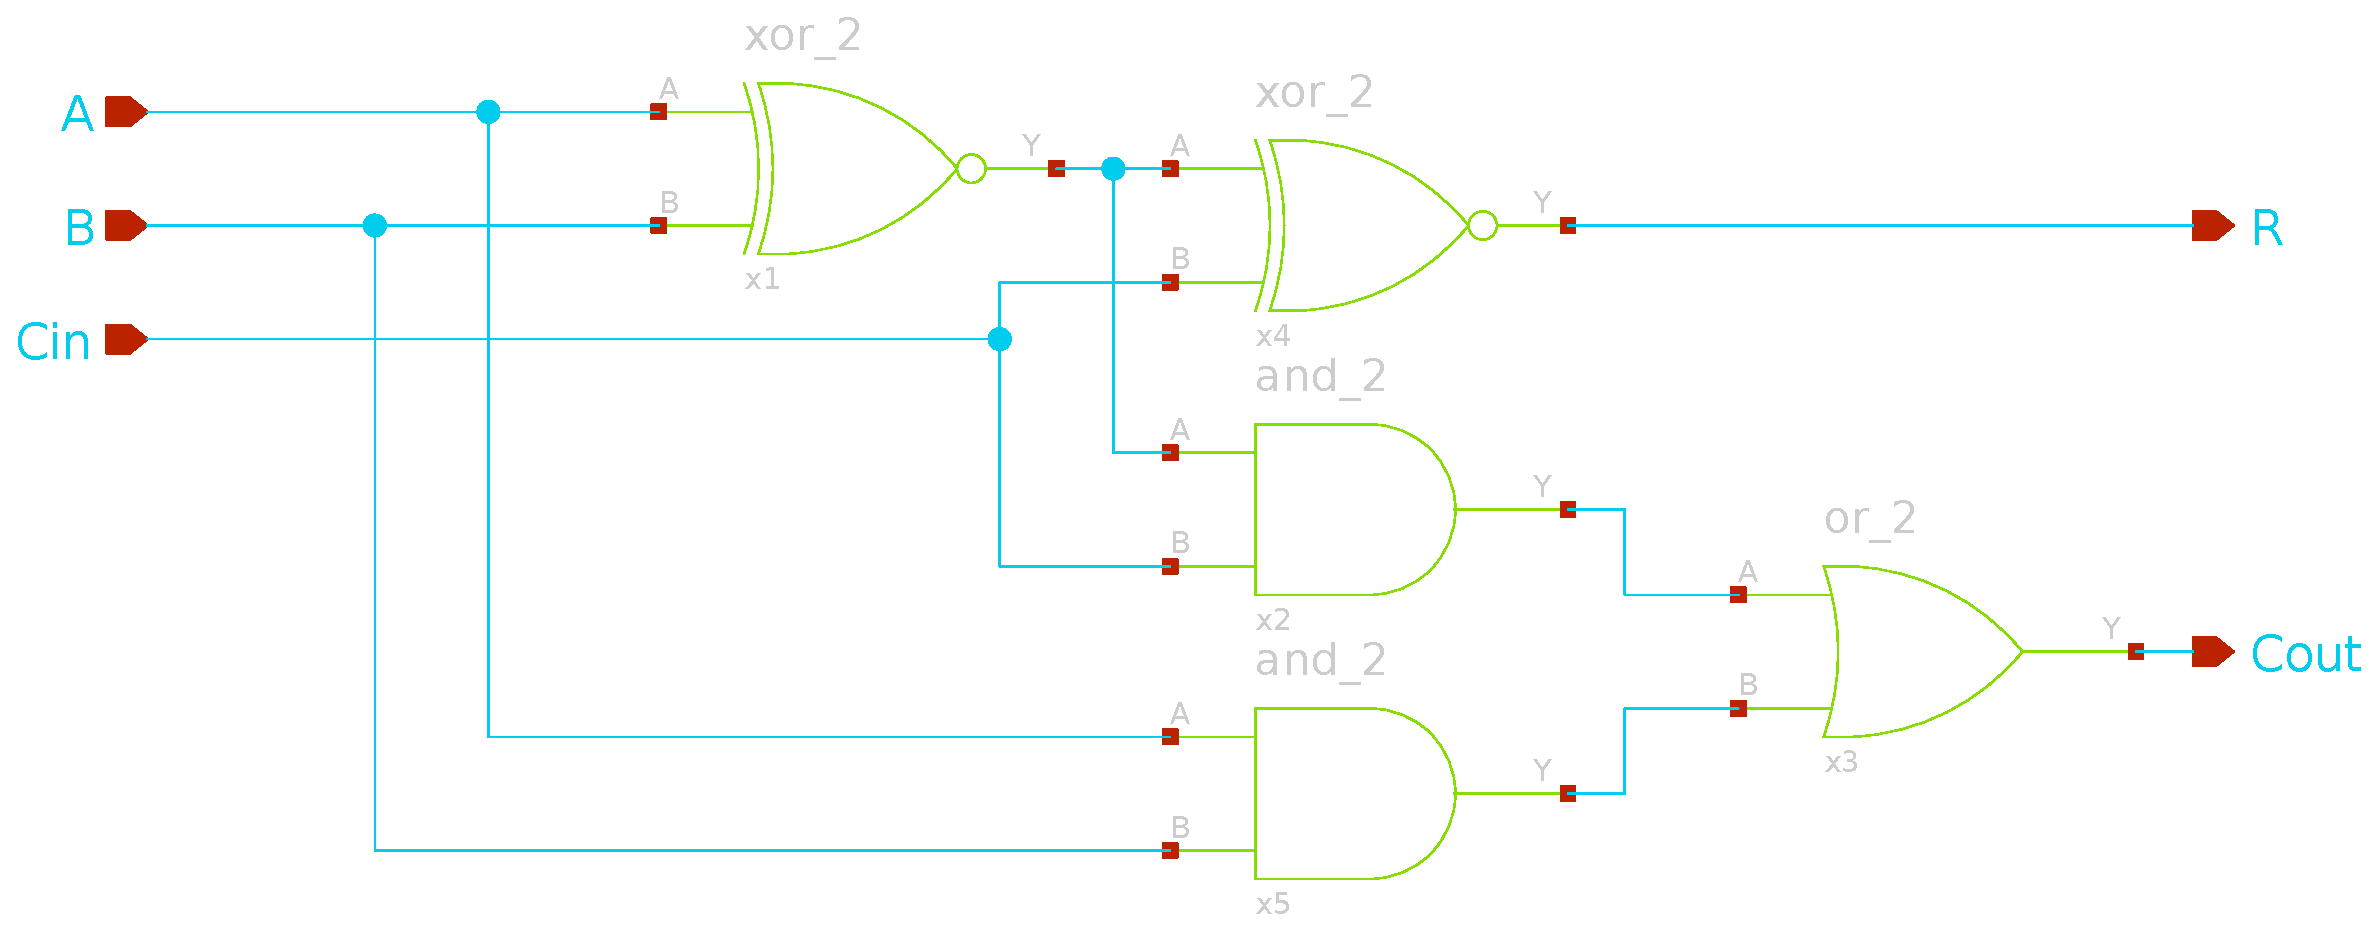
\includegraphics[width=\linewidth]{Immagini/full-adder}
			\caption{}
		\end{subfigure}
		\caption{rappresentazione simbolica del blocco half adder (a) e relativa implementazione mediante gate logici (b).}
		\label{fig:fa:sch}
	\end{figure}
	
	La cascata di circuiti xor (componenti \texttt{x1} e \texttt{x2}) permette di determinare univocamente il risultato $R$ del bit corrente, in quanto determinerà un valore logico alto in uscita solamente se un numero dispari di ingressi fossero anch'essi posti ad alta tensione.
	
	La definizione del riporto in uscita $C_{out}$ prevede invece la considerazione di due casi: se gli ingressi $A,B$ fossero stati logici alti, allora automaticamente il riporto in uscita dovrà essere posto ad alta tensione, e tale funzione è realizzata mediante il gate and \texttt{x5}. Una seconda casistica da considerare è quella complementare per cui la somma tra $A$ e $B$ non generasse riporto, ma potrebbe generarla la somma insieme al riporto in ingresso. Questo caso è analizzato dal gate and \texttt{x2} per cui gli ingressi sono il carry-in e il risultato della somma bit-a-bit degli ingressi (ottenuta dal gate xor \texttt{x1}). Il carry-out è dunque alto se almeno una delle due situazioni descritte è verificata.
	
	
\subsection*{Sommatore binario a 4 bit}
	Avendo appena descritto l'elemento circuitale alla base della somma di due bit distinti (con eventuale riporto in ingresso), è possibile realizzare uno schematico che permette la somma di due dati in forma binaria tramite la concatenazione dei full adder, come si può osservare in figura \ref{fig:add:sch}.
	
	\begin{figure}[bht]
		\centering
		\includegraphics[width=11cm]{Immagini/4bitadder}
		\caption{implementazione di un sommatore binario a 4 bit.}
		\label{fig:add:sch}
	\end{figure}
	
	In questo caso i segnali di input sono i numeri binari $A$ e $B$, oltre ad un eventuale riporto in ingresso $C_{in}$ (che può essere utilizzato per fare la somma di numeri a più bit rispetto all'architettura del sistema o può essere utilizzato rispetto alla codifica \textit{1 complementare} dei numeri binari) mentre l'uscita è determinata dai bit del risultato $R$ e dal riporto in uscita $C_{out}$. Come nel caso del contatore, il suffisso numerico 1 indica il bit meno significativo, mentre 4 il bit più significativo.
	
	Effettuare una simulazione completa di tutte le possibili combinazioni di ingresso (che sono in totale $16^2=256$) diventa praticamente difficile da effettuare ma soprattutto da visualizzare, per questo all'interno del documento viene mostrata una casistica rappresentativa ottenuta fissando un addendo e facendo variare l'altro.

	\begin{figure}[bht]
		\centering
		% GNUPLOT: LaTeX picture with Postscript
\begingroup
  \makeatletter
  \providecommand\color[2][]{%
    \GenericError{(gnuplot) \space\space\space\@spaces}{%
      Package color not loaded in conjunction with
      terminal option `colourtext'%
    }{See the gnuplot documentation for explanation.%
    }{Either use 'blacktext' in gnuplot or load the package
      color.sty in LaTeX.}%
    \renewcommand\color[2][]{}%
  }%
  \providecommand\includegraphics[2][]{%
    \GenericError{(gnuplot) \space\space\space\@spaces}{%
      Package graphicx or graphics not loaded%
    }{See the gnuplot documentation for explanation.%
    }{The gnuplot epslatex terminal needs graphicx.sty or graphics.sty.}%
    \renewcommand\includegraphics[2][]{}%
  }%
  \providecommand\rotatebox[2]{#2}%
  \@ifundefined{ifGPcolor}{%
    \newif\ifGPcolor
    \GPcolorfalse
  }{}%
  \@ifundefined{ifGPblacktext}{%
    \newif\ifGPblacktext
    \GPblacktexttrue
  }{}%
  % define a \g@addto@macro without @ in the name:
  \let\gplgaddtomacro\g@addto@macro
  % define empty templates for all commands taking text:
  \gdef\gplbacktext{}%
  \gdef\gplfronttext{}%
  \makeatother
  \ifGPblacktext
    % no textcolor at all
    \def\colorrgb#1{}%
    \def\colorgray#1{}%
  \else
    % gray or color?
    \ifGPcolor
      \def\colorrgb#1{\color[rgb]{#1}}%
      \def\colorgray#1{\color[gray]{#1}}%
      \expandafter\def\csname LTw\endcsname{\color{white}}%
      \expandafter\def\csname LTb\endcsname{\color{black}}%
      \expandafter\def\csname LTa\endcsname{\color{black}}%
      \expandafter\def\csname LT0\endcsname{\color[rgb]{1,0,0}}%
      \expandafter\def\csname LT1\endcsname{\color[rgb]{0,1,0}}%
      \expandafter\def\csname LT2\endcsname{\color[rgb]{0,0,1}}%
      \expandafter\def\csname LT3\endcsname{\color[rgb]{1,0,1}}%
      \expandafter\def\csname LT4\endcsname{\color[rgb]{0,1,1}}%
      \expandafter\def\csname LT5\endcsname{\color[rgb]{1,1,0}}%
      \expandafter\def\csname LT6\endcsname{\color[rgb]{0,0,0}}%
      \expandafter\def\csname LT7\endcsname{\color[rgb]{1,0.3,0}}%
      \expandafter\def\csname LT8\endcsname{\color[rgb]{0.5,0.5,0.5}}%
    \else
      % gray
      \def\colorrgb#1{\color{black}}%
      \def\colorgray#1{\color[gray]{#1}}%
      \expandafter\def\csname LTw\endcsname{\color{white}}%
      \expandafter\def\csname LTb\endcsname{\color{black}}%
      \expandafter\def\csname LTa\endcsname{\color{black}}%
      \expandafter\def\csname LT0\endcsname{\color{black}}%
      \expandafter\def\csname LT1\endcsname{\color{black}}%
      \expandafter\def\csname LT2\endcsname{\color{black}}%
      \expandafter\def\csname LT3\endcsname{\color{black}}%
      \expandafter\def\csname LT4\endcsname{\color{black}}%
      \expandafter\def\csname LT5\endcsname{\color{black}}%
      \expandafter\def\csname LT6\endcsname{\color{black}}%
      \expandafter\def\csname LT7\endcsname{\color{black}}%
      \expandafter\def\csname LT8\endcsname{\color{black}}%
    \fi
  \fi
    \setlength{\unitlength}{0.0500bp}%
    \ifx\gptboxheight\undefined%
      \newlength{\gptboxheight}%
      \newlength{\gptboxwidth}%
      \newsavebox{\gptboxtext}%
    \fi%
    \setlength{\fboxrule}{0.5pt}%
    \setlength{\fboxsep}{1pt}%
\begin{picture}(5668.00,3968.00)%
    \gplgaddtomacro\gplbacktext{%
      \csname LTb\endcsname%%
      \put(434,3322){\makebox(0,0)[r]{\strut{}$0$}}%
      \csname LTb\endcsname%%
      \put(434,3594){\makebox(0,0)[r]{\strut{}$0.9$}}%
      \csname LTb\endcsname%%
      \put(434,3866){\makebox(0,0)[r]{\strut{}$1.8$}}%
      \csname LTb\endcsname%%
      \put(566,3041){\makebox(0,0){\strut{}}}%
      \csname LTb\endcsname%%
      \put(1168,3041){\makebox(0,0){\strut{}}}%
      \csname LTb\endcsname%%
      \put(1770,3041){\makebox(0,0){\strut{}}}%
      \csname LTb\endcsname%%
      \put(2372,3041){\makebox(0,0){\strut{}}}%
      \csname LTb\endcsname%%
      \put(2975,3041){\makebox(0,0){\strut{}}}%
      \csname LTb\endcsname%%
      \put(3577,3041){\makebox(0,0){\strut{}}}%
      \csname LTb\endcsname%%
      \put(4179,3041){\makebox(0,0){\strut{}}}%
      \csname LTb\endcsname%%
      \put(4781,3041){\makebox(0,0){\strut{}}}%
      \csname LTb\endcsname%%
      \put(5383,3041){\makebox(0,0){\strut{}}}%
    }%
    \gplgaddtomacro\gplfronttext{%
      \csname LTb\endcsname%%
      \put(-171,3594){\rotatebox{-270}{\makebox(0,0){\strut{}$C_{out}$}}}%
      \put(2974,2975){\makebox(0,0){\strut{}}}%
    }%
    \gplgaddtomacro\gplbacktext{%
      \csname LTb\endcsname%%
      \put(434,2655){\makebox(0,0)[r]{\strut{}$0$}}%
      \csname LTb\endcsname%%
      \put(434,2928){\makebox(0,0)[r]{\strut{}$0.9$}}%
      \csname LTb\endcsname%%
      \put(434,3200){\makebox(0,0)[r]{\strut{}$1.8$}}%
      \csname LTb\endcsname%%
      \put(566,2375){\makebox(0,0){\strut{}}}%
      \csname LTb\endcsname%%
      \put(1168,2375){\makebox(0,0){\strut{}}}%
      \csname LTb\endcsname%%
      \put(1770,2375){\makebox(0,0){\strut{}}}%
      \csname LTb\endcsname%%
      \put(2372,2375){\makebox(0,0){\strut{}}}%
      \csname LTb\endcsname%%
      \put(2975,2375){\makebox(0,0){\strut{}}}%
      \csname LTb\endcsname%%
      \put(3577,2375){\makebox(0,0){\strut{}}}%
      \csname LTb\endcsname%%
      \put(4179,2375){\makebox(0,0){\strut{}}}%
      \csname LTb\endcsname%%
      \put(4781,2375){\makebox(0,0){\strut{}}}%
      \csname LTb\endcsname%%
      \put(5383,2375){\makebox(0,0){\strut{}}}%
    }%
    \gplgaddtomacro\gplfronttext{%
      \csname LTb\endcsname%%
      \put(-171,2927){\rotatebox{-270}{\makebox(0,0){\strut{}$R_4$}}}%
      \put(2974,2309){\makebox(0,0){\strut{}}}%
    }%
    \gplgaddtomacro\gplbacktext{%
      \csname LTb\endcsname%%
      \put(434,1989){\makebox(0,0)[r]{\strut{}$0$}}%
      \csname LTb\endcsname%%
      \put(434,2261){\makebox(0,0)[r]{\strut{}$0.9$}}%
      \csname LTb\endcsname%%
      \put(434,2533){\makebox(0,0)[r]{\strut{}$1.8$}}%
      \csname LTb\endcsname%%
      \put(566,1708){\makebox(0,0){\strut{}}}%
      \csname LTb\endcsname%%
      \put(1168,1708){\makebox(0,0){\strut{}}}%
      \csname LTb\endcsname%%
      \put(1770,1708){\makebox(0,0){\strut{}}}%
      \csname LTb\endcsname%%
      \put(2372,1708){\makebox(0,0){\strut{}}}%
      \csname LTb\endcsname%%
      \put(2975,1708){\makebox(0,0){\strut{}}}%
      \csname LTb\endcsname%%
      \put(3577,1708){\makebox(0,0){\strut{}}}%
      \csname LTb\endcsname%%
      \put(4179,1708){\makebox(0,0){\strut{}}}%
      \csname LTb\endcsname%%
      \put(4781,1708){\makebox(0,0){\strut{}}}%
      \csname LTb\endcsname%%
      \put(5383,1708){\makebox(0,0){\strut{}}}%
    }%
    \gplgaddtomacro\gplfronttext{%
      \csname LTb\endcsname%%
      \put(-171,2261){\rotatebox{-270}{\makebox(0,0){\strut{}$R_3$}}}%
      \put(2974,1642){\makebox(0,0){\strut{}}}%
    }%
    \gplgaddtomacro\gplbacktext{%
      \csname LTb\endcsname%%
      \put(434,1322){\makebox(0,0)[r]{\strut{}$0$}}%
      \csname LTb\endcsname%%
      \put(434,1594){\makebox(0,0)[r]{\strut{}$0.9$}}%
      \csname LTb\endcsname%%
      \put(434,1866){\makebox(0,0)[r]{\strut{}$1.8$}}%
      \csname LTb\endcsname%%
      \put(566,1041){\makebox(0,0){\strut{}}}%
      \csname LTb\endcsname%%
      \put(1168,1041){\makebox(0,0){\strut{}}}%
      \csname LTb\endcsname%%
      \put(1770,1041){\makebox(0,0){\strut{}}}%
      \csname LTb\endcsname%%
      \put(2372,1041){\makebox(0,0){\strut{}}}%
      \csname LTb\endcsname%%
      \put(2975,1041){\makebox(0,0){\strut{}}}%
      \csname LTb\endcsname%%
      \put(3577,1041){\makebox(0,0){\strut{}}}%
      \csname LTb\endcsname%%
      \put(4179,1041){\makebox(0,0){\strut{}}}%
      \csname LTb\endcsname%%
      \put(4781,1041){\makebox(0,0){\strut{}}}%
      \csname LTb\endcsname%%
      \put(5383,1041){\makebox(0,0){\strut{}}}%
    }%
    \gplgaddtomacro\gplfronttext{%
      \csname LTb\endcsname%%
      \put(-171,1594){\rotatebox{-270}{\makebox(0,0){\strut{}$R_2$}}}%
      \put(2974,975){\makebox(0,0){\strut{}}}%
    }%
    \gplgaddtomacro\gplbacktext{%
      \csname LTb\endcsname%%
      \put(434,656){\makebox(0,0)[r]{\strut{}$0$}}%
      \csname LTb\endcsname%%
      \put(434,928){\makebox(0,0)[r]{\strut{}$0.9$}}%
      \csname LTb\endcsname%%
      \put(434,1200){\makebox(0,0)[r]{\strut{}$1.8$}}%
      \csname LTb\endcsname%%
      \put(566,375){\makebox(0,0){\strut{}0}}%
      \csname LTb\endcsname%%
      \put(1168,375){\makebox(0,0){\strut{}100}}%
      \csname LTb\endcsname%%
      \put(1770,375){\makebox(0,0){\strut{}200}}%
      \csname LTb\endcsname%%
      \put(2372,375){\makebox(0,0){\strut{}300}}%
      \csname LTb\endcsname%%
      \put(2975,375){\makebox(0,0){\strut{}400}}%
      \csname LTb\endcsname%%
      \put(3577,375){\makebox(0,0){\strut{}500}}%
      \csname LTb\endcsname%%
      \put(4179,375){\makebox(0,0){\strut{}600}}%
      \csname LTb\endcsname%%
      \put(4781,375){\makebox(0,0){\strut{}700}}%
      \csname LTb\endcsname%%
      \put(5383,375){\makebox(0,0){\strut{}800}}%
    }%
    \gplgaddtomacro\gplfronttext{%
      \csname LTb\endcsname%%
      \put(-171,928){\rotatebox{-270}{\makebox(0,0){\strut{}$R_1$}}}%
      \put(2974,45){\makebox(0,0){\strut{}tempo $[ns]$}}%
    }%
    \gplbacktext
    \put(0,0){\includegraphics[width={283.40bp},height={198.40bp}]{Immagini/4bit-adder-sim}}%
    \gplfronttext
  \end{picture}%
\endgroup


		\caption{simulazione sul funzionamento del circuito di somma binaria. I grafici evidenziano l'andamento temporale dell'uscita dovuto alla somma di un ingresso costante $B=3_{10}=0011_{2}$ e un ingresso $A$ variabile da $0_{10}=0000_2$ a $15_{10}=1111_2$ che viene incrementato ogni $50ns$. Ogni uscita è collegata a massa mediante una capacità di carico di $0.75pF$. Le tensioni sono misurate in volt. }
		\label{fig:add:sim}
	\end{figure}
	
	Considerando la simulazione in figura \ref{fig:add:sim} dove si suppone un ingresso costante (in questo caso $B=3_{10}=0011_2$) è possibile valutare la risposta del circuito per le 16 combinazioni in ingresso del segnale $A$ considerando che lo stesso aumenta di un'unità ogni $50ns$. Per esempio considerando l'intervallo di tempo di $300-350ns$ associato ad un ingresso $A=6_{10}=0110_2$, si osserva che il risultato della somma è dato dai bit
	\[ R = R_4R_3R_2R_1 = 1001_2 = 9_{10} \qquad, \qquad C_{out} = 0 \]
	Si verifica dunque il funzionamento del circuito. Si osserva inoltre che per i tempi $t > 650ns$ ($A\geq 13_{10}$) il riporto in uscita $C_{out}$ commuta allo stato logico alto: questo comportamento risulta essere corretto in quanto numeri a 4 bit possono rappresentare solamente 16 numeri decimali (da 0 a 15). Le uscite per cui $A\geq 13_{10}$ (essendo $B=3_{10}$) determinano una somma che è fuori dal range di rappresentazione a 4 bit, per questo viene posto ad alto il riporto in uscita (che si può considerare come il quinto bit più significativo del risultato) e i bit di risultato $R_i$ lavorano come di consueto. Utilizzando $C_{out}$ come quinto bit significativo è possibile verificare anche le somme per $A\geq 13_{10}$: considerando come esempio l'ultimo ingresso $A = 15_{10}=1111_2$ (per $t\in [750,800]ns$) l'uscita del circuito è data dall'espressione
	\[ R = C_{out}R_4R_3R_2R_1 = 10010_2 = 18_{10} \]
	
	
\section{Moltiplicatore binario}
	L'operazione di moltiplicazione binaria è una delle funzioni più complesse da realizzare a livello hardware, in quanto richiede la presenza di un numero elevato di componenti o svariati cicli di clock per svolgere l'operazione matematica. La moltiplicazione può essere effettuata secondo diverse metodologie che possono essere sia di tipo algoritmico (sfruttando una procedura che utilizza circuito sommatore e registri a scorrimento) oppure implementate a livello hardware.
	
	In questo caso si farà riferimento a quest'ultima metodologia, in quanto più immediata da analizzare. Per capire come effettuare l'operazione è necessario schematizzare il funzionamento richiesto effettuando manualmente un'operazione di moltiplicazione binaria, dove in questo caso si utilizza un moltiplicando $a$ a 4 bit e un moltiplicatore $b$ di 3 bit.
	
	\begin{center}
	\begin{tabular}{ c c c c c c c}
		&&$a_4$ & $a_3$ & $a_2$ & $a_1$ & $\times$ \\ 
		&&& $b_3$ & $b_2$ & $b_1$ & $=$ \\ \hline		 
		&&$a_4b_1$ & $a_3b_1$ & $a_2b_1$ & $a_1b_1$ & $+$ \\ 
		&$a_4b_2$ & $a_3b_2$ & $a_2b_2$ & $a_1b_2$ & & $+$ \\
		$a_4b_3$ & $a_3b_3$ & $a_2b_3$ & $a_1b_3$ &&& $=$ \\ \hline
		$a_4b_3$ & $a_4b_2+a_3b_3$ & $a_4b_1+a_3b_2a_2b_3$ & $a_3b_1 + a_2b_2a_1b_3$ & $a_2b_1+a_1b_2$ & $a_1b_1$& $=$ 	
	\end{tabular} 
	\end{center}
	
	I vari termini ottenuti nelle somme parziali sono determinati direttamente dal prodotto logico di due bit, e dunque possono essere determinati (a livello circuitale) velocemente mediante gate and. A questo punto è invece necessario effettuare la somma binaria delle varie somme parziali, considerando che le stesse devono essere \textit{spostate a sinistra} di un'unità ad ogni iterazione (come viene effettuato normalmente nel prodotto decimale ed è rappresentato nella tabella riassuntiva).
	
	\begin{figure}[bht]
		\centering
		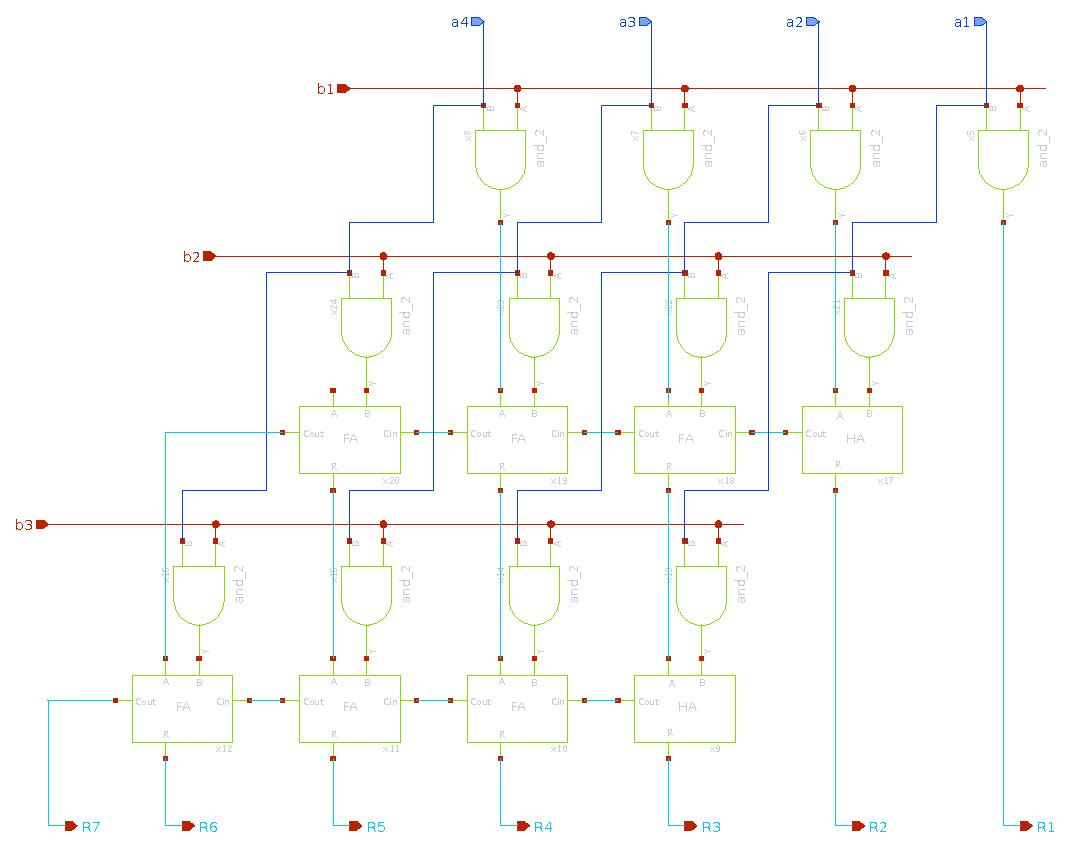
\includegraphics[width=\linewidth]{Immagini/moltiplicatore}
		\caption{implementazione circuitale di un moltiplicatore binario con moltiplicando a 4 bit e moltiplicatore a 3 bit. }
		\label{fig:molt:sch}
	\end{figure}
	
	In figura \ref{fig:molt:sch} è mostrato il circuito combinatorio che realizza l'operazione di moltiplicazione binaria mediante l'utilizzo di gate and oltre che al circuito half adder (HA) e full adder (FA); le interconnessioni in blu rappresentano il percorso degli ingressi del moltiplicando nel circuito, mentre in rosso sono evidenziati i bit del moltiplicatore.
	
	I problemi legati ad un'implementazione in tecnologia c-mos, come così mostrata, è che richiede un'elevata quantità di risorse hardware intese come numero di transistor e dunque spazio su chip. Considerando infatti un moltiplicando di $n$ bit e un moltiplicatore di $m$ bit, allora il numero di linee di circuiti di addizione è pari a $m-1$ (con $n$ full/half adder l'una) e l'uscita può richiedere l'utilizzo fino a $n+m$ bit. Lo schematico risulta essere "compatto" per valori di $m,n$ sufficientemente piccoli (in questo caso $m=4,n=3$), tuttavia in sistemi reali dove può essere necessario effettuare operazioni tra dati a $16$ bit o più, l'impatto risulta essere importante.
	
	\paragraph{Simulazione} Come nel caso del circuito sommatore, testare esaustivamente tutte le possibili combinazioni d'ingresso risulta complesso, tuttavia è possibile mostrare la correttezza di funzionamento del circuito fissando un parametro e facendo variare l'altro termine. In figura \ref{fig:molt:sim} è mostrata una simulazione nel dominio del tempo fissando a $5_{10}$ il moltiplicando e facendo variare da $0$ a $7$ il moltiplicatore.
	
	\begin{figure}[p]
		\centering
		% GNUPLOT: LaTeX picture with Postscript
\begingroup
  \makeatletter
  \providecommand\color[2][]{%
    \GenericError{(gnuplot) \space\space\space\@spaces}{%
      Package color not loaded in conjunction with
      terminal option `colourtext'%
    }{See the gnuplot documentation for explanation.%
    }{Either use 'blacktext' in gnuplot or load the package
      color.sty in LaTeX.}%
    \renewcommand\color[2][]{}%
  }%
  \providecommand\includegraphics[2][]{%
    \GenericError{(gnuplot) \space\space\space\@spaces}{%
      Package graphicx or graphics not loaded%
    }{See the gnuplot documentation for explanation.%
    }{The gnuplot epslatex terminal needs graphicx.sty or graphics.sty.}%
    \renewcommand\includegraphics[2][]{}%
  }%
  \providecommand\rotatebox[2]{#2}%
  \@ifundefined{ifGPcolor}{%
    \newif\ifGPcolor
    \GPcolorfalse
  }{}%
  \@ifundefined{ifGPblacktext}{%
    \newif\ifGPblacktext
    \GPblacktexttrue
  }{}%
  % define a \g@addto@macro without @ in the name:
  \let\gplgaddtomacro\g@addto@macro
  % define empty templates for all commands taking text:
  \gdef\gplbacktext{}%
  \gdef\gplfronttext{}%
  \makeatother
  \ifGPblacktext
    % no textcolor at all
    \def\colorrgb#1{}%
    \def\colorgray#1{}%
  \else
    % gray or color?
    \ifGPcolor
      \def\colorrgb#1{\color[rgb]{#1}}%
      \def\colorgray#1{\color[gray]{#1}}%
      \expandafter\def\csname LTw\endcsname{\color{white}}%
      \expandafter\def\csname LTb\endcsname{\color{black}}%
      \expandafter\def\csname LTa\endcsname{\color{black}}%
      \expandafter\def\csname LT0\endcsname{\color[rgb]{1,0,0}}%
      \expandafter\def\csname LT1\endcsname{\color[rgb]{0,1,0}}%
      \expandafter\def\csname LT2\endcsname{\color[rgb]{0,0,1}}%
      \expandafter\def\csname LT3\endcsname{\color[rgb]{1,0,1}}%
      \expandafter\def\csname LT4\endcsname{\color[rgb]{0,1,1}}%
      \expandafter\def\csname LT5\endcsname{\color[rgb]{1,1,0}}%
      \expandafter\def\csname LT6\endcsname{\color[rgb]{0,0,0}}%
      \expandafter\def\csname LT7\endcsname{\color[rgb]{1,0.3,0}}%
      \expandafter\def\csname LT8\endcsname{\color[rgb]{0.5,0.5,0.5}}%
    \else
      % gray
      \def\colorrgb#1{\color{black}}%
      \def\colorgray#1{\color[gray]{#1}}%
      \expandafter\def\csname LTw\endcsname{\color{white}}%
      \expandafter\def\csname LTb\endcsname{\color{black}}%
      \expandafter\def\csname LTa\endcsname{\color{black}}%
      \expandafter\def\csname LT0\endcsname{\color{black}}%
      \expandafter\def\csname LT1\endcsname{\color{black}}%
      \expandafter\def\csname LT2\endcsname{\color{black}}%
      \expandafter\def\csname LT3\endcsname{\color{black}}%
      \expandafter\def\csname LT4\endcsname{\color{black}}%
      \expandafter\def\csname LT5\endcsname{\color{black}}%
      \expandafter\def\csname LT6\endcsname{\color{black}}%
      \expandafter\def\csname LT7\endcsname{\color{black}}%
      \expandafter\def\csname LT8\endcsname{\color{black}}%
    \fi
  \fi
    \setlength{\unitlength}{0.0500bp}%
    \ifx\gptboxheight\undefined%
      \newlength{\gptboxheight}%
      \newlength{\gptboxwidth}%
      \newsavebox{\gptboxtext}%
    \fi%
    \setlength{\fboxrule}{0.5pt}%
    \setlength{\fboxsep}{1pt}%
\begin{picture}(6802.00,6802.00)%
    \gplgaddtomacro\gplbacktext{%
      \csname LTb\endcsname%%
      \put(548,5991){\makebox(0,0)[r]{\strut{}$0$}}%
      \csname LTb\endcsname%%
      \put(548,6325){\makebox(0,0)[r]{\strut{}$0.9$}}%
      \csname LTb\endcsname%%
      \put(548,6658){\makebox(0,0)[r]{\strut{}$1.8$}}%
      \csname LTb\endcsname%%
      \put(680,5697){\makebox(0,0){\strut{}}}%
      \csname LTb\endcsname%%
      \put(1403,5697){\makebox(0,0){\strut{}}}%
      \csname LTb\endcsname%%
      \put(2125,5697){\makebox(0,0){\strut{}}}%
      \csname LTb\endcsname%%
      \put(2848,5697){\makebox(0,0){\strut{}}}%
      \csname LTb\endcsname%%
      \put(3570,5697){\makebox(0,0){\strut{}}}%
      \csname LTb\endcsname%%
      \put(4293,5697){\makebox(0,0){\strut{}}}%
      \csname LTb\endcsname%%
      \put(5015,5697){\makebox(0,0){\strut{}}}%
      \csname LTb\endcsname%%
      \put(5738,5697){\makebox(0,0){\strut{}}}%
      \csname LTb\endcsname%%
      \put(6460,5697){\makebox(0,0){\strut{}}}%
    }%
    \gplgaddtomacro\gplfronttext{%
      \csname LTb\endcsname%%
      \put(-57,6324){\rotatebox{-270}{\makebox(0,0){\strut{}$R_7$}}}%
      \put(3570,5631){\makebox(0,0){\strut{}}}%
    }%
    \gplgaddtomacro\gplbacktext{%
      \csname LTb\endcsname%%
      \put(548,5175){\makebox(0,0)[r]{\strut{}$0$}}%
      \csname LTb\endcsname%%
      \put(548,5509){\makebox(0,0)[r]{\strut{}$0.9$}}%
      \csname LTb\endcsname%%
      \put(548,5842){\makebox(0,0)[r]{\strut{}$1.8$}}%
      \csname LTb\endcsname%%
      \put(680,4881){\makebox(0,0){\strut{}}}%
      \csname LTb\endcsname%%
      \put(1403,4881){\makebox(0,0){\strut{}}}%
      \csname LTb\endcsname%%
      \put(2125,4881){\makebox(0,0){\strut{}}}%
      \csname LTb\endcsname%%
      \put(2848,4881){\makebox(0,0){\strut{}}}%
      \csname LTb\endcsname%%
      \put(3570,4881){\makebox(0,0){\strut{}}}%
      \csname LTb\endcsname%%
      \put(4293,4881){\makebox(0,0){\strut{}}}%
      \csname LTb\endcsname%%
      \put(5015,4881){\makebox(0,0){\strut{}}}%
      \csname LTb\endcsname%%
      \put(5738,4881){\makebox(0,0){\strut{}}}%
      \csname LTb\endcsname%%
      \put(6460,4881){\makebox(0,0){\strut{}}}%
    }%
    \gplgaddtomacro\gplfronttext{%
      \csname LTb\endcsname%%
      \put(-57,5508){\rotatebox{-270}{\makebox(0,0){\strut{}$R_6$}}}%
      \put(3570,4815){\makebox(0,0){\strut{}}}%
    }%
    \gplgaddtomacro\gplbacktext{%
      \csname LTb\endcsname%%
      \put(548,4359){\makebox(0,0)[r]{\strut{}$0$}}%
      \csname LTb\endcsname%%
      \put(548,4693){\makebox(0,0)[r]{\strut{}$0.9$}}%
      \csname LTb\endcsname%%
      \put(548,5026){\makebox(0,0)[r]{\strut{}$1.8$}}%
      \csname LTb\endcsname%%
      \put(680,4065){\makebox(0,0){\strut{}}}%
      \csname LTb\endcsname%%
      \put(1403,4065){\makebox(0,0){\strut{}}}%
      \csname LTb\endcsname%%
      \put(2125,4065){\makebox(0,0){\strut{}}}%
      \csname LTb\endcsname%%
      \put(2848,4065){\makebox(0,0){\strut{}}}%
      \csname LTb\endcsname%%
      \put(3570,4065){\makebox(0,0){\strut{}}}%
      \csname LTb\endcsname%%
      \put(4293,4065){\makebox(0,0){\strut{}}}%
      \csname LTb\endcsname%%
      \put(5015,4065){\makebox(0,0){\strut{}}}%
      \csname LTb\endcsname%%
      \put(5738,4065){\makebox(0,0){\strut{}}}%
      \csname LTb\endcsname%%
      \put(6460,4065){\makebox(0,0){\strut{}}}%
    }%
    \gplgaddtomacro\gplfronttext{%
      \csname LTb\endcsname%%
      \put(-57,4692){\rotatebox{-270}{\makebox(0,0){\strut{}$R_5$}}}%
      \put(3570,3999){\makebox(0,0){\strut{}}}%
    }%
    \gplgaddtomacro\gplbacktext{%
      \csname LTb\endcsname%%
      \put(548,3543){\makebox(0,0)[r]{\strut{}$0$}}%
      \csname LTb\endcsname%%
      \put(548,3877){\makebox(0,0)[r]{\strut{}$0.9$}}%
      \csname LTb\endcsname%%
      \put(548,4210){\makebox(0,0)[r]{\strut{}$1.8$}}%
      \csname LTb\endcsname%%
      \put(680,3249){\makebox(0,0){\strut{}}}%
      \csname LTb\endcsname%%
      \put(1403,3249){\makebox(0,0){\strut{}}}%
      \csname LTb\endcsname%%
      \put(2125,3249){\makebox(0,0){\strut{}}}%
      \csname LTb\endcsname%%
      \put(2848,3249){\makebox(0,0){\strut{}}}%
      \csname LTb\endcsname%%
      \put(3570,3249){\makebox(0,0){\strut{}}}%
      \csname LTb\endcsname%%
      \put(4293,3249){\makebox(0,0){\strut{}}}%
      \csname LTb\endcsname%%
      \put(5015,3249){\makebox(0,0){\strut{}}}%
      \csname LTb\endcsname%%
      \put(5738,3249){\makebox(0,0){\strut{}}}%
      \csname LTb\endcsname%%
      \put(6460,3249){\makebox(0,0){\strut{}}}%
    }%
    \gplgaddtomacro\gplfronttext{%
      \csname LTb\endcsname%%
      \put(-57,3876){\rotatebox{-270}{\makebox(0,0){\strut{}$R_4$}}}%
      \put(3570,3183){\makebox(0,0){\strut{}}}%
    }%
    \gplgaddtomacro\gplbacktext{%
      \csname LTb\endcsname%%
      \put(548,2726){\makebox(0,0)[r]{\strut{}$0$}}%
      \csname LTb\endcsname%%
      \put(548,3060){\makebox(0,0)[r]{\strut{}$0.9$}}%
      \csname LTb\endcsname%%
      \put(548,3394){\makebox(0,0)[r]{\strut{}$1.8$}}%
      \csname LTb\endcsname%%
      \put(680,2432){\makebox(0,0){\strut{}}}%
      \csname LTb\endcsname%%
      \put(1403,2432){\makebox(0,0){\strut{}}}%
      \csname LTb\endcsname%%
      \put(2125,2432){\makebox(0,0){\strut{}}}%
      \csname LTb\endcsname%%
      \put(2848,2432){\makebox(0,0){\strut{}}}%
      \csname LTb\endcsname%%
      \put(3570,2432){\makebox(0,0){\strut{}}}%
      \csname LTb\endcsname%%
      \put(4293,2432){\makebox(0,0){\strut{}}}%
      \csname LTb\endcsname%%
      \put(5015,2432){\makebox(0,0){\strut{}}}%
      \csname LTb\endcsname%%
      \put(5738,2432){\makebox(0,0){\strut{}}}%
      \csname LTb\endcsname%%
      \put(6460,2432){\makebox(0,0){\strut{}}}%
    }%
    \gplgaddtomacro\gplfronttext{%
      \csname LTb\endcsname%%
      \put(-57,3060){\rotatebox{-270}{\makebox(0,0){\strut{}$R_3$}}}%
      \put(3570,2366){\makebox(0,0){\strut{}}}%
    }%
    \gplgaddtomacro\gplbacktext{%
      \csname LTb\endcsname%%
      \put(548,1910){\makebox(0,0)[r]{\strut{}$0$}}%
      \csname LTb\endcsname%%
      \put(548,2244){\makebox(0,0)[r]{\strut{}$0.9$}}%
      \csname LTb\endcsname%%
      \put(548,2578){\makebox(0,0)[r]{\strut{}$1.8$}}%
      \csname LTb\endcsname%%
      \put(680,1616){\makebox(0,0){\strut{}}}%
      \csname LTb\endcsname%%
      \put(1403,1616){\makebox(0,0){\strut{}}}%
      \csname LTb\endcsname%%
      \put(2125,1616){\makebox(0,0){\strut{}}}%
      \csname LTb\endcsname%%
      \put(2848,1616){\makebox(0,0){\strut{}}}%
      \csname LTb\endcsname%%
      \put(3570,1616){\makebox(0,0){\strut{}}}%
      \csname LTb\endcsname%%
      \put(4293,1616){\makebox(0,0){\strut{}}}%
      \csname LTb\endcsname%%
      \put(5015,1616){\makebox(0,0){\strut{}}}%
      \csname LTb\endcsname%%
      \put(5738,1616){\makebox(0,0){\strut{}}}%
      \csname LTb\endcsname%%
      \put(6460,1616){\makebox(0,0){\strut{}}}%
    }%
    \gplgaddtomacro\gplfronttext{%
      \csname LTb\endcsname%%
      \put(-57,2244){\rotatebox{-270}{\makebox(0,0){\strut{}$R_2$}}}%
      \put(3570,1550){\makebox(0,0){\strut{}}}%
    }%
    \gplgaddtomacro\gplbacktext{%
      \csname LTb\endcsname%%
      \put(548,1094){\makebox(0,0)[r]{\strut{}$0$}}%
      \csname LTb\endcsname%%
      \put(548,1428){\makebox(0,0)[r]{\strut{}$0.9$}}%
      \csname LTb\endcsname%%
      \put(548,1762){\makebox(0,0)[r]{\strut{}$1.8$}}%
      \csname LTb\endcsname%%
      \put(680,800){\makebox(0,0){\strut{}0}}%
      \csname LTb\endcsname%%
      \put(1403,800){\makebox(0,0){\strut{}100}}%
      \csname LTb\endcsname%%
      \put(2125,800){\makebox(0,0){\strut{}200}}%
      \csname LTb\endcsname%%
      \put(2848,800){\makebox(0,0){\strut{}300}}%
      \csname LTb\endcsname%%
      \put(3570,800){\makebox(0,0){\strut{}400}}%
      \csname LTb\endcsname%%
      \put(4293,800){\makebox(0,0){\strut{}500}}%
      \csname LTb\endcsname%%
      \put(5015,800){\makebox(0,0){\strut{}600}}%
      \csname LTb\endcsname%%
      \put(5738,800){\makebox(0,0){\strut{}700}}%
      \csname LTb\endcsname%%
      \put(6460,800){\makebox(0,0){\strut{}800}}%
    }%
    \gplgaddtomacro\gplfronttext{%
      \csname LTb\endcsname%%
      \put(-57,1428){\rotatebox{-270}{\makebox(0,0){\strut{}$R_1$}}}%
      \put(3570,470){\makebox(0,0){\strut{}tempo $[ns]$}}%
    }%
    \gplbacktext
    \put(0,0){\includegraphics[width={340.10bp},height={340.10bp}]{Immagini/mult-sim}}%
    \gplfronttext
  \end{picture}%
\endgroup


		\caption{bit in uscita ottenuti mediante la moltiplicazione di un moltiplicando costante pari a $0101_2=5_{10}$ e un moltiplicatore che incrementa ogni $100ns$ di una unità dal valore $0000_2=0_{10}$ al valore $1111_2=15_{10}$. Tutte le uscite sono collegate a massa mediante una capacità di carico di $0.75pF$. Le tensioni sono espresse in volt. }
		\label{fig:molt:sim}
	\end{figure}
	
	\paragraph{Glitch} Nella pratica i segnali analogici non si propagano istantaneamente e seguendo una legge prettamente analitica, ma prevedono un contributo stocastico e dunque non prevedibile a priori. La realizzazione pratica, come già affermato, comporta inevitabilmente l'introduzione di capacità parassite spesso non quantificabili, introducendo delle inerzie alla trasmissione del segnale.
	
	Sono proprio questi fenomeni (che il pdk tenta di modellare) che danno origine ai cosiddetti \textit{glitch}, ossia delle corse critiche che portano ad un movimento temporaneo dell'uscita rispetto al valore desiderato per via del ritardo degli ingressi. Un esempio di questo fenomeno è ben visibile al tempo $t=400ns$ per i bit $R_3$ ed $R_6$ in figura \ref{fig:molt:sim} (ma in generale ogni commutazione, anche nei circuiti precedenti, è soggetta a questo tipo di problema), dove il ritardo nella propagazione a cascata dei segnali attraverso i vari gate introduce dei ritardi per i quali l'uscita tende a commutare nonostante debba rimanere costante.
	
	Questi fenomeni, inevitabili nella pratica, sono tendenzialmente di durata irrisoria (rispetto al caso appena indicato il tempo di ripristino è inferiore a $12ns$): per questo nei circuiti ad applicazione digitale non si considera mai come ingresso il segnale al tempo di clock (dove si ha la trasmissione delle uscite ai vari circuiti a valle), ma si aspetta un tempo consono per esaurire i transitori dei circuiti e gli eventuali glitch.
	
	
	
	